\documentclass{DEIThesis}
\usepackage{booktabs}
\usepackage{textcomp}

\title{Panorama energetico italiano: guidare una transizione sostenibile}

\author{Matteo Garbo}
\studentId{142841}

% Advisor
\advisor{Prof. Savino Stefano}

\university{Università di Udine}
\mastername{Ingegneria Gestionale}
\academicYear{2021/2022}

\begin{filecontents*}[overwrite]{\jobname.xmpdata}
    \Title{An interesting title for the thesis}
    \Author{Luca Martinelli}
    \Language{en-EN}
    \Keywords{Computer Engineering\sep LaTeX}
\end{filecontents*}

% Document

\begin{document}
    % The front matter (Cover, ToC, Abstract, etc...)
    \frontmatter

    % The main content
    \mainmatter
    
    %!TEX root = ../main.tex

\chapter{Introduzione}
\label{chp:intro}
Questa tesi si pone l'obiettivo di trattare diversi ambiti del campo energetico: si parte con la definizione di fonte energetica cioè: \enquote{Una qualsiasi sostanza, materiale o fenomeno naturale o artificiale che può essere utilizzato per produrre energia}.
Partendo da questa si è effettuata una divisione per capire quali energie avessero una natura rinnovabile e quali invece non rinnovabile.
\begin{figure}[H]
    \centering
    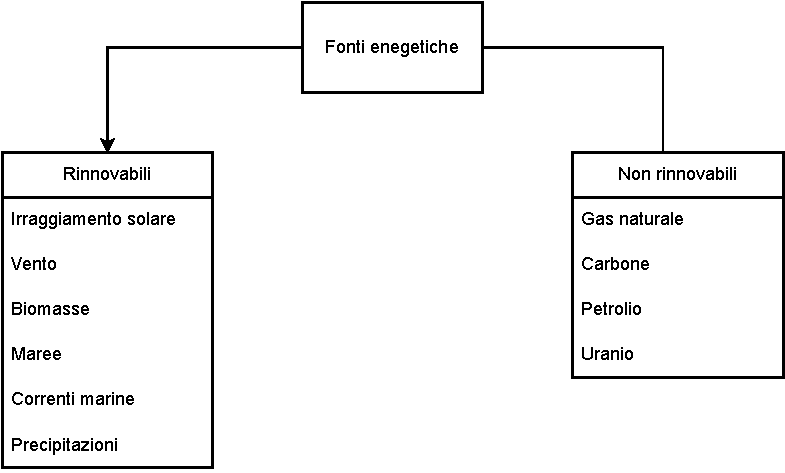
\includegraphics[height=0.4\textwidth]{res/cap 1/diagramma intro}
    \caption{Diagramma della prima suddivisione delle fonti energetiche}
\end{figure}\noindent
Si procede poi con una descrizione dettagliata prima delle fonti rinnovabili andando a definire la loro origine, le proprietà energetiche ed eventuali problematiche o accortezze che devono essere note per sfruttarle.\\
Si prosegue con una descrizione delle fonti partendo da quelle rinnovabili e descrivendo i fenomeni naturali che ne danno origine per poi procedere con la stesa metodologia con quelle non rinnovabili.\\
Il capitolo successivo tratterà gli impianti utilizzati per sfruttare le fonti precedentemente citate: in questo caso verranno trattati solo gli impianti rinnovabili in quanto di maggior interesse per quest'elaborato.
Per ciascun impianto saranno descritti i punti salienti che ne permettono l'applicazione, per ciascuna fonte potrebbero essere presenti più tipologie di impianti in tal caso saranno descritte singolarmente per metterne il luce le differenze.
\newpage
\begin{wrapfigure}{l}{5.5cm}
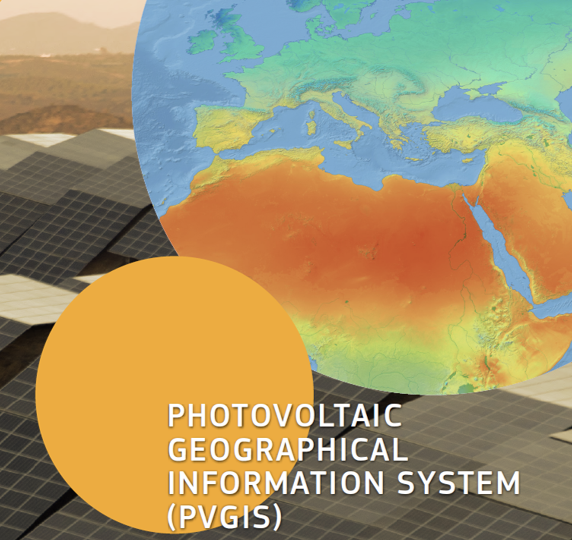
\includegraphics[width=5.5cm]{res/cap 1/PVGIS tool}
\end{wrapfigure} 
Per introdurre il caso studio che questa tesi si propone di illustrare, mi servirò di un tool offerto dal Joint Research Centre chiamato PVGIS: un capitolo ne tratterà l'accurata descrizione per trasmettere al lettore le potenzialità di tale strumento.
Questo, infatti, permette sia di effettuare in automatico calcoli sulla produzioni di diverse tipologie di impianti che di esportare dati grezzi da rielaborare poi con strumenti esterni.\\
Lo studio che condurrò come conclusione di questo elaborato sarà mirato a evidenziare le differenze costruttive che un impianto fotovoltaico riscontra in diverse locazioni geografiche e quanto le caratteristiche di esse, pur essendo alla stessa longitudine, ne influenzino la produzione.
\par
Le scelte delle collocazione degli impianti saranno effettuate cercando di evitare che il loro funzionamento sia alterato da condizioni meteo anomale per la regione o che siano influenzate dalla morfologia del territorio.
    %!TEX root = ../main.tex

\chapter{Fonti energetiche}
\label{chp:FontiEnergetiche}
Quando si parla di fonti energetiche, queste possono essere suddivise in fonti rinnovabile e fonti non rinnovabili. Per ciascuna delle due categorie, nel corso dell'elaborato, verranno elencati i vari tipi di impianti utilizzati per sfruttarle trasformandole in energia. 

\section{Fonti rinnovabili}
Sono considerate fonti rinnovabili tutte quelle provenienti da:
\begin{itemize}
    \item Irraggiamento solare
    \item Vento
    \item Biomasse
    \item Maree
    \item Correnti marine
    \item Precipitazioni
\end{itemize}
\subsection{Irraggiamento solare}

La radiazione solare è l'energia emessa dal sole, generata a partire da reazioni termonucleari di fusione che avvengono nel sole producendo radiazioni elettromagnetiche a diversa frequenza e lunghezza d'onda le quali trasportano l'energia solare.\\
La radiazione solare che raggiunge il livello più alto dell'atmosfera terrestre è mediamente \(1367\frac{W}{m^2}\), chiamata costante solare (\textit{S}).\\
\textit{S} rappresenta la quantità di energia trasmessa ad un disco di diametro uguale a quello terrestre posto tangenzialmente al livello più alto dell'atmosfera.
%Essendo però la terra assimilabile ad una sfera che ruota attorno al proprio asse,per ottenere il valore medio per unità di tempo di radiazioni che arriva su di essa bisogna quindi considerarne la superficie esterna arrivando ad un valore medio di circa 342$\frac{W}{m^2}$\footnote{Valore considerato sempre nel livello superiore dell'atmosfera}.\\
\newpage\noindent
In buona approssimazione considerando\cite{captazione-enegia-solare}:
\begin{itemize}
    \item fenomeni di riflessione dati dalle nuvole
    \item fenomeni di riflessione dati dalle polveri presenti in atmosfera
    \item fenomeni di interazione chimica con i gas presenti in atmosfera
    \item fenomeni di scattering
\end{itemize}
A causa dei fenomeni elencati sopra,le radiazioni solari che arrivano al suolo presentano quindi due componenti:
\begin{itemize}
    \item diretta, cioè la componente che raggiunge il suolo senza venir in alcun modo perturbata e quindi con la stessa direzione del sole.
    \item diffusa, costituita dalla componente che raggiunge il suolo dopo essere stata dispersa,assorbita ed eventualmente re-irraggiata.
\end{itemize}
La presenza delle due componenti risulta di fondamentale importanza durante il processo di captazione e va tenuta in considerazione durante la scelta della tipologia di impianto da installare, argomento che verrà trattato nel capitolo successivo.\\
L'industria statunitense in collaborazione con l'ASTM\footnote{American Society for Testing and Materials} ha definito tre standard:
\begin{enumerate}
    \item AM0
    \item AM1.5-f
    \item AM1-37$^\circ$
\end{enumerate}
Prima di concentrarci sulla spiegazione di questi è importante definire un valore m, tale da rispettare la seguente proporzione matematica $m=\frac{1}{\cos z}$, come si evince nella figura sottostante:
\begin{figure}[H]
    \centering
    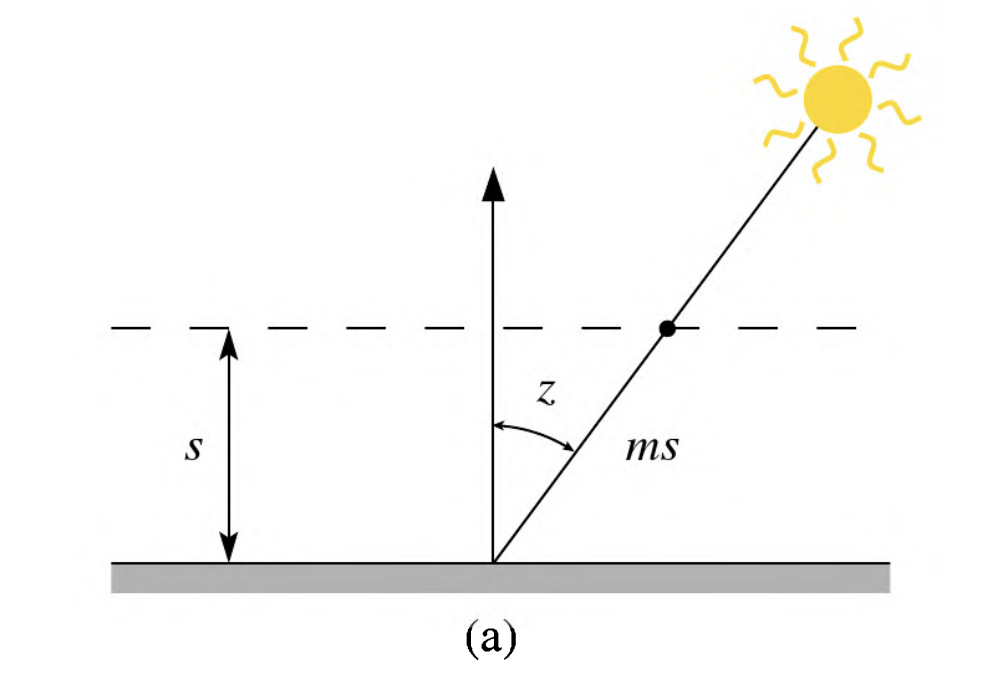
\includegraphics[width=0.4\textwidth]{res/cap 2/rappresentazione m.png}
    \caption{Percorso delle radiazioni solari}
\end{figure}
Il primo standard fa riferimento all'irradianza nel livello più alto dell'atmosfera,
gli altri invece all'irradianza che giunge al suolo dopo un percorso di lunghezza m = 1,5 in un'atmosfera limpida, dove per limpida si considera una visibilità di 23 km.
La seconda fa nello specifico riferimento ad una superficie $A_n$ ortogonale ai raggi solari,la seconda fa riferimento ad una superficie $A_i$ rivolta a sud ed inclinata di un'angolo $\beta = 37^\circ$ rispetto al piano orizzontale, nell'impotesi di un coefficiente di riflessione $\rho_s = 0,2$.
\begin{figure}[H]
    \centering
    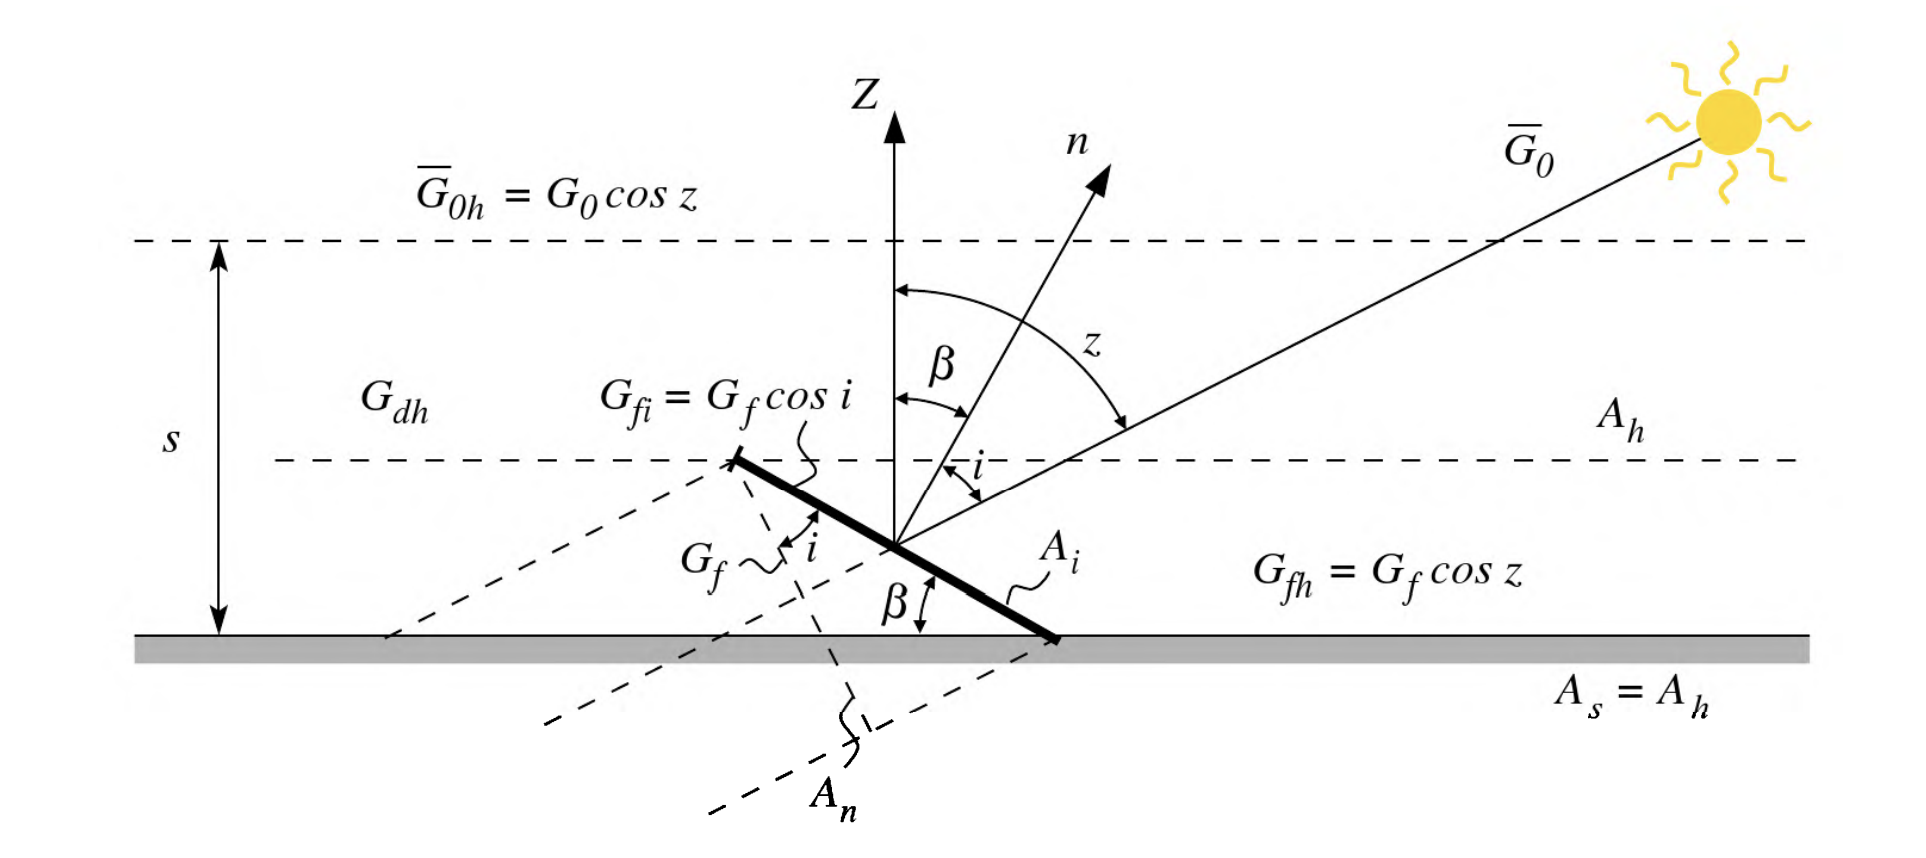
\includegraphics[width=0.8\textwidth]{res/cap 2/standard.png}
    \caption{Rappresentazione superfici stanadard AM1.5-f AM1-37$^\circ$}
\end{figure}
L'energia trasportata dalle radiazioni solari possiamo dividerla sostanzialmente in due componenti:
\begin{itemize}
    \item \textbf{Componente visibile:} quella con lunghezza d'onda [\textbf{$\lambda$}] tra i 400 ed i 700 nm
    \item \textbf{Componenti ad energia minoritaria:} 
        \begin{itemize}
            \item \textbf{ultravioletti} \textbf{$\lambda$} tra i 100 ed i 400nm
            \item \textbf{infrarossi} \textbf{$\lambda$} tra i 700nm ed 1mm
        \end{itemize}
\end{itemize}
Successivamente, questa ulteriore suddivisione ci sarà utile per spiegare alcune tecnologie che sono in grado di lavorare sulle singole componenti.
\begin{figure}[H]
    \centering
    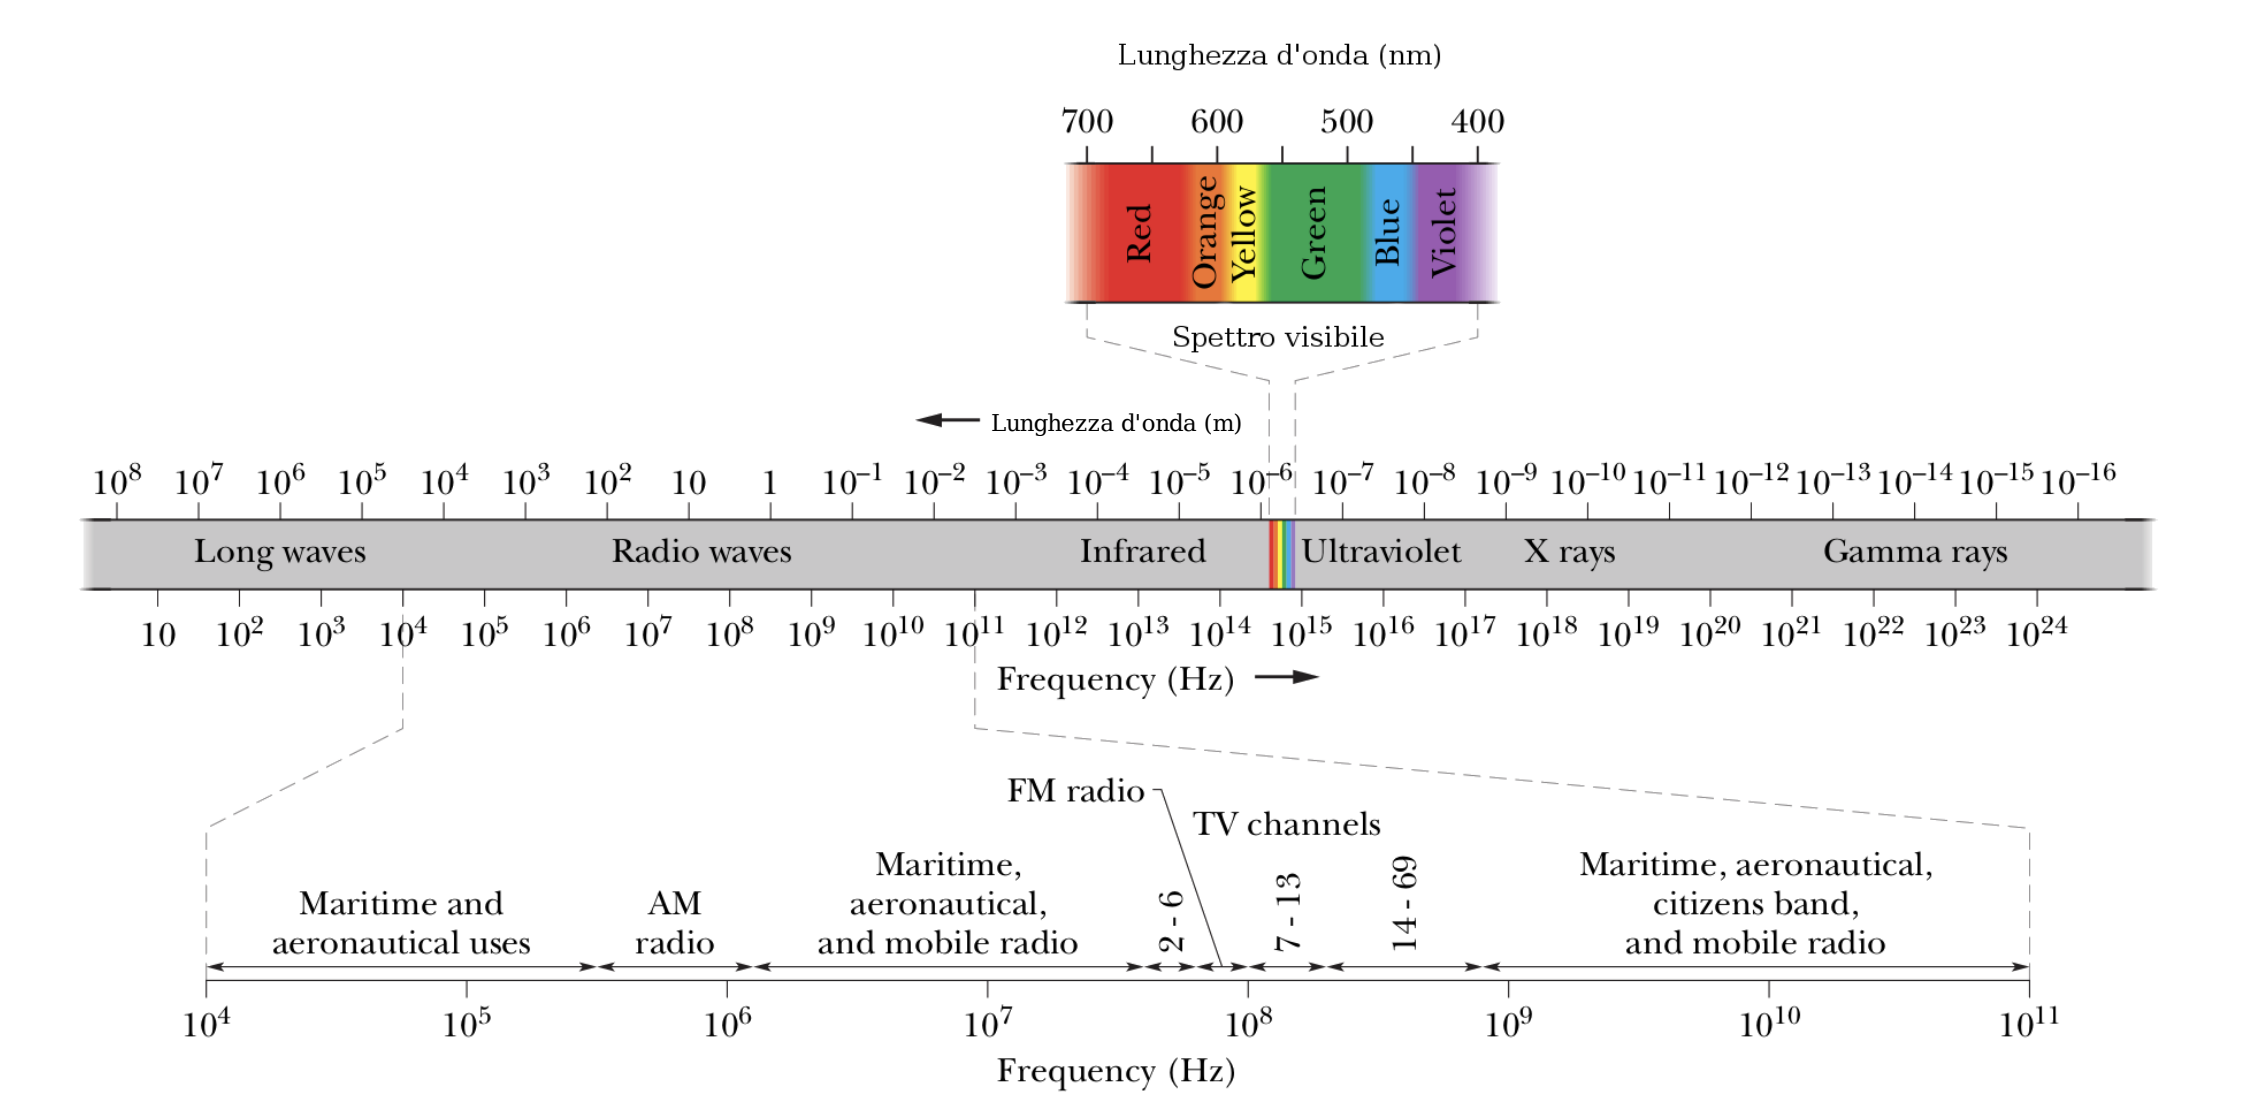
\includegraphics[width=0.8\textwidth]{res/cap 2/luce_dettagli.png}
    \caption{Radiazione solare}
\end{figure}

\newpage
\subsection{Vento}

Ciò che comunemente viene chiamato vento, è il movimento di una massa d'aria da una regione ad alta pressione ad una a bassa pressione.\\
Quando si parla di vento ci sono diversi aspetti da considerare quali:
\begin{itemize}
    \item Velocità
    \item Densità della massa d'aria
    \item Contenuto energetico
\end{itemize}
\noindent 
Con contenuto energetico si intente l'energia cinetica che l'aria ha in movimento:
\begin{center}
    \large{\(E=\frac{1}{2}\cdot m\cdot v^2 = \frac{1}{2} \cdot(Avt\rho)\cdot v^2 = \frac{1}{2} \cdot(Avt\rho)\cdot v^2 \)}
\end{center}
\noindent
Possiamo notare come, sia l'energia cinetica che la massa d'aria considerata, dipendono da tutti i parametri sopra elencati. Capire il modo in cui essi partecipano al bilancio energetico, ci permetterà nei capitoli successivi, di comprendere il funzionamento degli impianti eolici.

\subsection{Biomasse}
Con biomasse intendiamo tutta quella serie di prodotti organici usati per produrre calore o elettricità in specifici impianti appositamente progettate.\\
Sono classificabili in base al fatto che vengano o meno prodotte per generare energia elettrica\cite{IRENA}:
\begin{itemize}
    \item Biomasse primarie
    \item Biomasse secondarie
\end{itemize}
\noindent
Nella prime categoria inseriamo tutto il materiale organico prodotto con lo specifico scopo energetico, mentre, nella seconda vengono inseriti tutti i prodotti organici che sono il risultato di scarti residenziali ed industriali.

\vspace{2mm}
Adesso che abbiamo specificato tutto ciò che è considerabile biomassa andiamo ad elencare le tecniche utilizzate per sfruttare l'energia potenziale contenuta in esse\cite{EIA2022}:
\begin{description}[labelindent=5mm]
    \item[$\bullet$ Conversione termica]: questa tipologia si procede tramite un riscaldamento della biomassa con lo scopo di produrre combustibili in vario stato. Nella categoria sono state inserite tre tecniche che vanno a loro volta a generate combustibili in diverso stato:
    \begin{description}[labelindent=5mm]
        \item[$\cdot$ Torrefazione:] processo che prevede il riscaldamento della biomassa ad una temperatura compresa tra i 200 ed i 300\degree C in un ambiente quasi privo di ossigeno, dalla biomassa vengono rimosse le componenti a contenuto energetico più basso. Il 30\% viene quindi convertito in gas mentre la restante parte rimane sotto forma di bricchetti solidi o pellet mantenendo però circa l'85\% dell'energia originaria della biomassa\cite{Torrification}. 
        \item[$\cdot$ Pirolisi:] processo che comporta un riscaldamento dei materiali organici ad una temperatura tra i 400 ed i 500\degree C in quasi assenza di ossigeno. Le sostanze generate da questo processo sono: bio-oli, carbone, metano ed idrogeno.\\
        Partendo dal bio-olio e tramite un successivo processo di idrotrattamento a temperatura e pressione elevata si possono produrre biocarburanti\cite{EIA2021}.
        \item[$\cdot$ Gassificazione:] processo, anch'esso che prevede un riscaldamento delle biomasse ad una temperatura compresa tra gli 800 ed i 900\degree C , questa volta però inserendo in modo controllato ossigeno e/o vapore acqueo con l'obbiettivo di produrre \enquote{syngas}, il quale potrà poi essere usato per scopi energetici.\cite{EIA2022}
    \end{description}
    \item[$\bullet$ Conversione chimica] questa categoria comprende una serie di processi chimici che hanno lo scopo di trasformare le biomasse in una forma più facile da trasportare ed immagazzinare.\\
    Molti di essi sono simili al processo per produrre \enquote{syngas} spiegato nel punto precedente, un esempio è un processo chiamato \enquote{transesterificazione} nel quale una sostanza organica viene fatta reagire con dell'alcool per produrre biocarburanti.\cite{EIA2022}
    \item[$\bullet$ Conversione biologica] nella sezione sono inseriti tutti quei processi che sfruttano microrganismi per un processo di conversione, tra questi si possono citare: digestione anaerobica, fermentazione e compostaggio.\\ Lo scopo è quello di trasformare la biomassa in sostanze quali bioetanolo o biogas. 
\end{description}

\subsection{Maree}
Le maree sono il naturale cambiamento del livello del mare causato da una combinazione di effetti gravitazionali della luna e del sole, legati alla rotazione terrestre.\\Il cambiamento di marea attraversa due stati fondamentali: quando il livello smette di diminuire raggiungendo un minimo locale ci troviamo in uno stato chiamato bassa marea, viceversa, quando smette di crescere raggiunge uno stato di massimo locale parliamo di alta marea.\\
Sono presenti,in prima approssimazione, due componenti fondamentali le quali poi avranno anch'esse delle componenti specifiche chiamati costituenti:\\

\vspace{0,5em}\noindent
\begin{center}
    

\begin{tabular}{|c|c|c|c|}
\hline
\multicolumn{4}{|l|}{Semi-diurna}\\
\hline
Costituente & Periodo(h) & Velocità($\degree$/h) & Ampiezza(cm) \\ 
\hline
M2  & 12.421 & 28.984 & 58  \\ \hline
S2  & 12 & 30 & 13.7  \\ \hline
N2  & 12.658 & 28.439 & 12.3  \\\hline
\end{tabular}\\

\vspace{1em}\noindent
\begin{tabular}{|c|c|c|c|}
\hline
\multicolumn{4}{|l|}{Diurna}\\
\hline
Costituente & Periodo(h) & Velocità($\degree$/h) & Ampiezza(cm) \\ 
\hline
K1  & 23.934 & 15.041 & 36.8 \\ \hline
O1  & 25.819 & 13.943 & 23.0 \\ \hline
P1 & 24.066 & 14.958 & 11.6 \\\hline
\end{tabular}\\
\end{center}
\vspace{1em}
\noindent
I dati riportati nelle tabelle soprastanti ci indicano le componenti principali riferite in una determinata posizione geografica presa come esempio. Sono state riportate solamente le principali in quanto, tramite esse, è possibile ottenere una buona approssimazione sull'andamento della marea\footnote{Dati ricavati dal sito del National Oceanic and Atmospheric Administration della città di San Francisco}.

\begin{figure}[H]
    \centering
    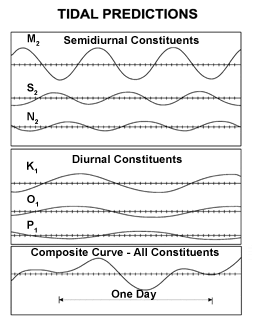
\includegraphics[width=0.3\textwidth]{res/cap 2/Tidal_constituent_sum.png}
    \caption{Curva ottenuta dai costituenti}
\end{figure}

Si nota come la curva ottenuta sia la somma delle componenti, essa rappresenta l'andamento della marea dato dalle componenti principali e più rilevanti.\\
Ci sono, inoltre, fattori che influenzano l'andamento delle maree che non dipendono solamente dai puri dati numerici sopra indicati correlati all'orario od alla stagione in cui ci si trova, ma anche dalla realtà geografica.\\
Il livello del mare nelle coste francesi mediterranee, ad esempio, oscilla meno di quanto avviene sulle coste francesi che danno sull'oceano in quanto la presenza di stretti non permette all'acqua di mantenere un andamento di discesa/salita lineare ma lo altera. Da qui la difficoltà maggiore di riuscire a creare un modello predittivo affidabile per realtà particolare quali la città di Venezia a esempio.
\subsection{Correnti marine}
Con corrente marina intendiamo una massa d'acqua in movimento rispetto a quella che la circonda e che può avere una differente densità,salinità o temperatura.\\
Gli effetti principali che provocano la formazione di queste correnti sono:\cite{NOAA-current}
\begin{itemize}
    \item Effetto di Coriolis
    \item Differenza di temperatura
    \item Differenza di salinità
    \item Rottura del moto ondoso
    \item \enquote{Cabbeling}
\end{itemize}\noindent
Si parla di \enquote{Cabbeling} quando abbiamo due basse d'acqua, denominate con A e B, andando a mescolarsi formeranno una nuova massa d'acqua che ha una densità superiore a quella di A e B.
\vfill
\newpage
\begin{figure}[H]
    \centering
    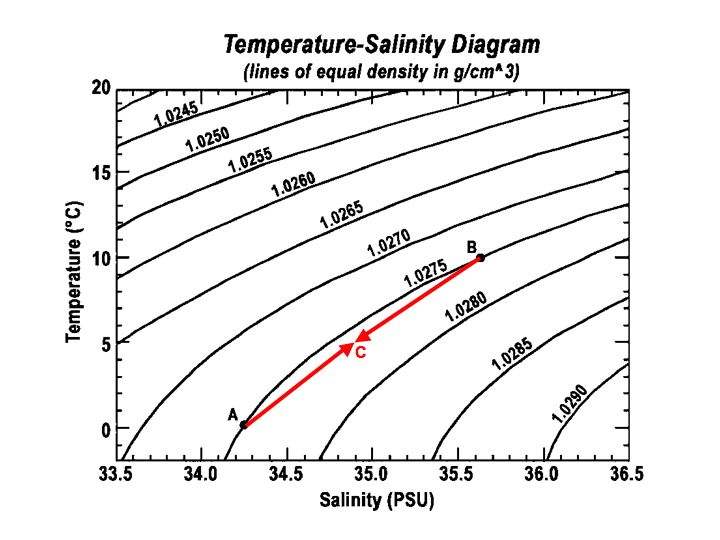
\includegraphics[width=0.5\textwidth]{res/cap 2/temperature-salinity}
    \caption{Diagramma Temperatura salinità ed effetto "Cabbeling"}
\end{figure}\noindent
La dinamica che descrive le varie correnti parte da una divisione dell'oceano in tre livelli:
\begin{itemize}
    \item \textbf{Strato misto:} è uno stato superficiale le cui proprietà fisiche variano nel tempo e le cui correnti sono generate dagli strati inferiori
    \item \textbf{Oceano superiore:} sopra la linea termoclina
    \item \textbf{Oceano profondo:}  sotto la linea termoclina
\end{itemize}\noindent
Con linea termoclina identifichiamo un livello nel quale avviene un'importante rimescolamento dell'acqua e nel quale c'è quindi una più veloce variazione di temperatura, un esempio si può vedere nel grafico riportato sotto:
\begin{figure}[H]
    \centering
    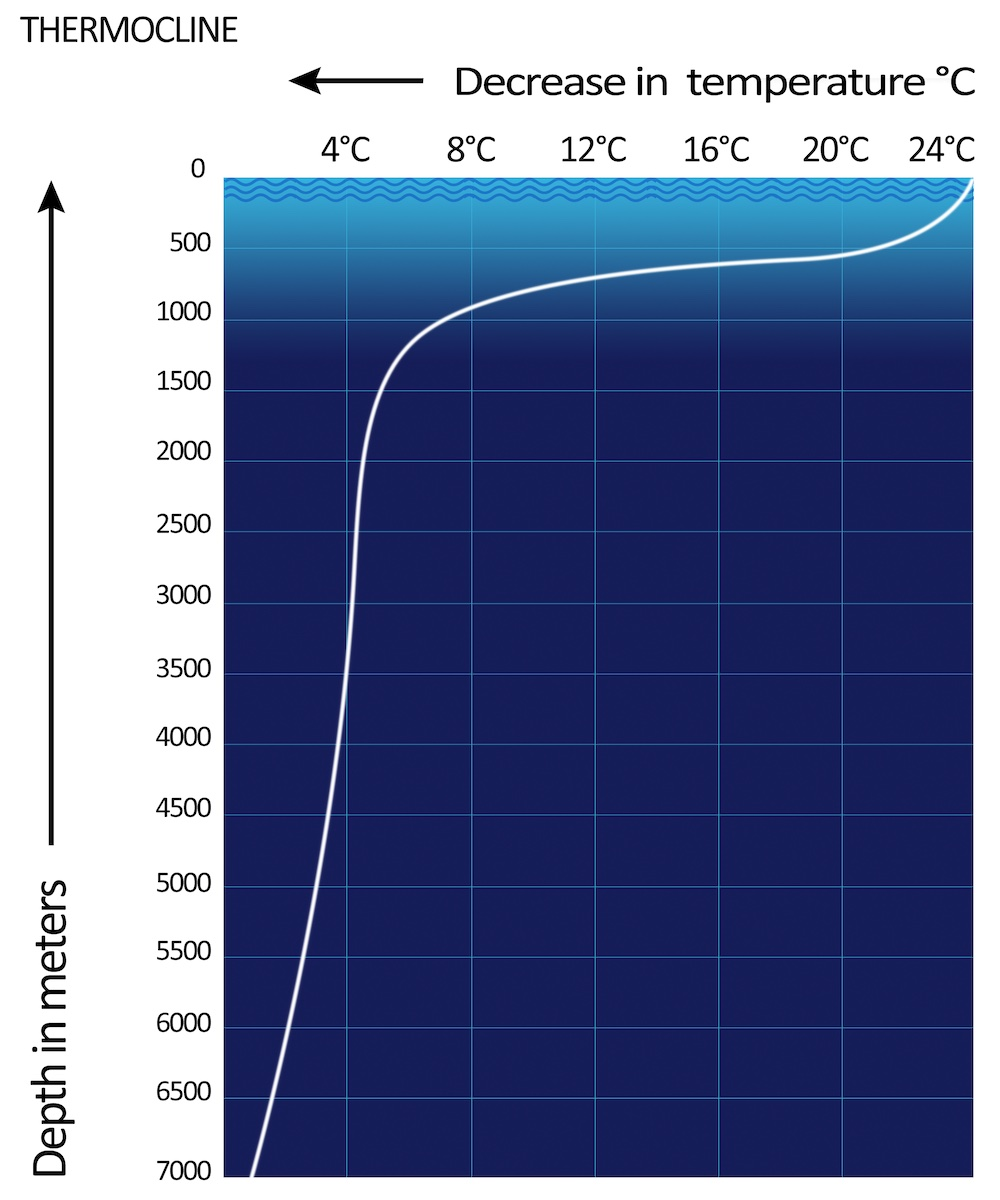
\includegraphics[height=0.4\textwidth]{res/cap 2/termoclino}
    \caption{Variazione di temperatura in funzione della profondità}
\end{figure}\noindent
Tutte le correnti oceaniche di superficie sono solitamente guidate da correnti ventose, venti che sono influenzati in gran parte dall'effetto di Coriolis sopra citato.\\
Le correnti più profonde sono mosse da un fenomeno chiamato: \enquote{Circolazione termoalina}.
Esso è a sua volte correlato a fenomeni fisici legati alla variazione di densità e di temperatura. I principali agenti che provocano una variazione di temperatura o densità sono il calore proveniente da livelli superiori e la differenza di densità provocata da grandi flussi d'acqua dolce provenienti sempre da i livelli superiori.\\

\subsection{Precipitazioni}
Le precipitazioni sono un fenomeno atmosferico che porta il vapore acqueo contenuto nell'atmosfera,una volta condensato, a cadere per l'effetto della gravità.\\
L'aria contiene vapore acqueo e la sua quantità varia molto da zona a zona e quindi non è comunemente inserita negli elementi che compongono l'aria.\\
Per esprimerne il quantitativo contenuto in atmosfera si usano diversi metodi:
\begin{itemize}
    \item Rapporto volumetrico: $(\frac{volume\,  d'acqua}{volume\,  d'aria})$
    \item Umidità specifica: rapporto in massa tra quantità di vapore e quantità di aria  $(\frac{g\, H_2O}{kg\, aria})$
    \item Mixing ratio: rapporto tra la quantità di vapore acqueo e quella d'aria secca $(\frac{g\, H_2O}{kg\, aria\, secca})$
    \item Umidità assoluta: densità di vapore acqueo $(\frac{g\, H_2O}{m^3\, aria})$
    \item Umidità relativa: rapporto tra la pressione parziale di acqua e la pressione di saturazione dell'acqua ad una determinata temperatura $(\frac{p_{H_2O} }{p_{H_2O}^s})\%$
\end{itemize}
L'incontro di masse d'aria aventi temperature diverse porterà quella a temperatura maggiore a salire generando una zona a bassa pressione, salendo la temperatura della massa calda e la pressione inizieranno a scendere fino a far incontrare al vapore condizioni che gli permettono di condensare e quindi di cadere a terra generando fenomeni di rovesci.\\
\newpage
\section{Fonti non rinnovabili}
Sono considerate non fonti rinnovabili:
\begin{itemize}
    \item Gas naturale
    \item Carbone
    \item Petrolio
    \item Uranio
\end{itemize}
Ad esclusione dell'uranio, per ciascuna delle fonti verrà fatto un breve excursus sulla formazione, sul potere calorifero che è in grado di offrire anche in relazione al suo prezzo di mercato. Verranno riportati i prezzi presi da un noto sito governativo già citato in precedenza presi tutti nello stesso periodo e opportunamente convertiti in unità per renderli confrontabili.\\
Parlando di prezzi, è importante precisare come quelli inseriti siano puramente indicativi e relativi ad un determinato mercato e non tengano conto di voci di costo importanti quali: gli impianti necessari a trasportarli e la importante differente strutturale e quindi di costo degli impianti di generazione.\\
\subsection{Gas naturale}
Quando si parla di gas naturale si indica una miscela di più gas:
\begin{itemize}
    \item Metano($C H_4$)
    \item Etano ($C_2 H_6$)
    \item Propano ($C_3 H_8$)
    \item Butano ($C_4 H_10$)
    \item Anidride carbonica ($C O_2$)
    \item Azoto ($N_2$)
    \item Ossigeno ($O_2$)
    \item Gas nobili(tracce)
\end{itemize}
Si può subito notare come il gas naturale non contenga solo idrocarburi ma anche altre sostanze, le quali vanno considerate sia durante il bilancio energetico che durante il trattamento degli inquinanti.\\
In prima analisi possiamo immaginare una combustione ideale di metano:
\begin{center}
    \ch{CH4\gas{} + 2 O2\gas{}->CO2\gas{} + 2 H2O\gas}
\end{center}
Per il calcolo dell'energia sprigionata dalla reazione useremo la legge di Hess la quale conoscendo tramite apposite tabelle i $\Delta H$ di formazione dei vari componenti ci permette di conoscere quella dell'intera reazione.
\begin{center}
    \large{$\Delta H_{rz} = \Delta H_{f,CO_2}(T) + 2\Delta H_{f,H_2O}(T) - \Delta H_{f,CH_4}(T) - \Delta H_{f,O_2}(T) $}
\end{center}
Sostituendo i valori ottenuti sperimentalmente e poi tabulati\footnote{https://cccbdb.nist.gov/xp1.asp?prop=1} otteniamo:
\begin{center}
    \large{$\Delta H_{rz} = -803070\frac{Kj}{Kmol} $}
\end{center}
A questo punto possiamo ottenere il potere energetico di un Kg di metano:
\begin{center}
    {\large$\frac{\Delta H_{rz}}{PM_{CH_4}} = \frac{-803070}{16.042} = -50060 \frac{Kj}{Kg} \sim -35.83 \frac{MJ}{Nm^3}$\footnote{Metro cubo normale(1atm e 0\degree C)}}
\end{center}
\newpage\noindent
Parlando di combustibili è importante citare due caratteristiche cioè:
\begin{itemize}
    \item Potere calorifero inferiore(LHV)
    \item Potere calorifero superiore(HHV)
\end{itemize}
\smallskip
\noindent
Il primo non tiene conto del calore latente di vaporizzazione dell'acqua generata durante la combustione mentre il secondo ne tiene conto.\\
E' importante esprimere entrambi i valori in quando, nei moderni impianti, si è in grado di utilizzare anche il delta energetico tra il limite superiore ed inferiore andando quindi a sfruttare meglio le risorse aumentando il rendimento.\\
Quello calcolato in precedenza avendo nella reazione l'acqua in uscita in forma gassosa corrisponde al LHV, per calcolare l'HHV bisogna tenere in considerazione la quantità di energia che va sottratta a al vapore per farlo condensare:
\begin{center}
    \large{$\Delta H = 2 \cdot -44010 = -88020 \frac{Kj}{Kmol} \Rightarrow \frac{-88020}{18.016}[\frac{\Delta H}{PM_{H_2O}}] = -4886 \frac{Kj}{Kg}$}
\end{center}
Sommando il valore ottenuto a quello precedentemente calcolato possiamo trovare l'HHV:
\begin{center}
    \normalsize{$HHV = \Delta H_{rz} + \Delta H_{cond} = -803070 + (-88020) = -891090 \frac{Kj}{Kmol}\sim -55547 \frac{Kj}{Kmol} \sim -39.76 \frac{MJ}{Nm^3}$}
\end{center}
Tutti i segni negativi sono dovuti al fatto che la reazione presa in considerazione sia esoergonica.\\
L'energia liberata sarà sotto forma di energia termica potrà poi essere opportunamente trasformata o direttamente utilizzata.\\
Il prezzo riportato per il gas naturale in questo caso è in $\frac{\$}{million BTU}$ ed equivale a 6,60\$ che riportandolo in unità del S.I. equivale a $0,0062\frac{\$}{MJ}$.\\
\subsection{Carbone}
Sono presenti diverse tipologie di carbone. Queste si differenziano inizialmente in fossili e non fossili.\\
Tra i carboni fossili troviamo:
\begin{itemize}
    \item Torba
    \item Lignite
    \item Litantrace
    \item Antracite
\end{itemize}
Si differenziano per una crescente percentuale di carbonio e per la diminuzione progressiva dell'umidità contenuta.\\
Per andare a proporre un bilancio energetico come per il gas naturale è stato anche qui necessario fare delle semplificazioni.\\
\vfill
\newpage
Il tutto è iniziato con un'analisi su quale fosse il carbone fossile maggiormente utilizzato negli anni per capire quale convenisse prendere in esame:\cite{EIA-Statistics-World}\\
\begin{figure}[H]
    \centering
    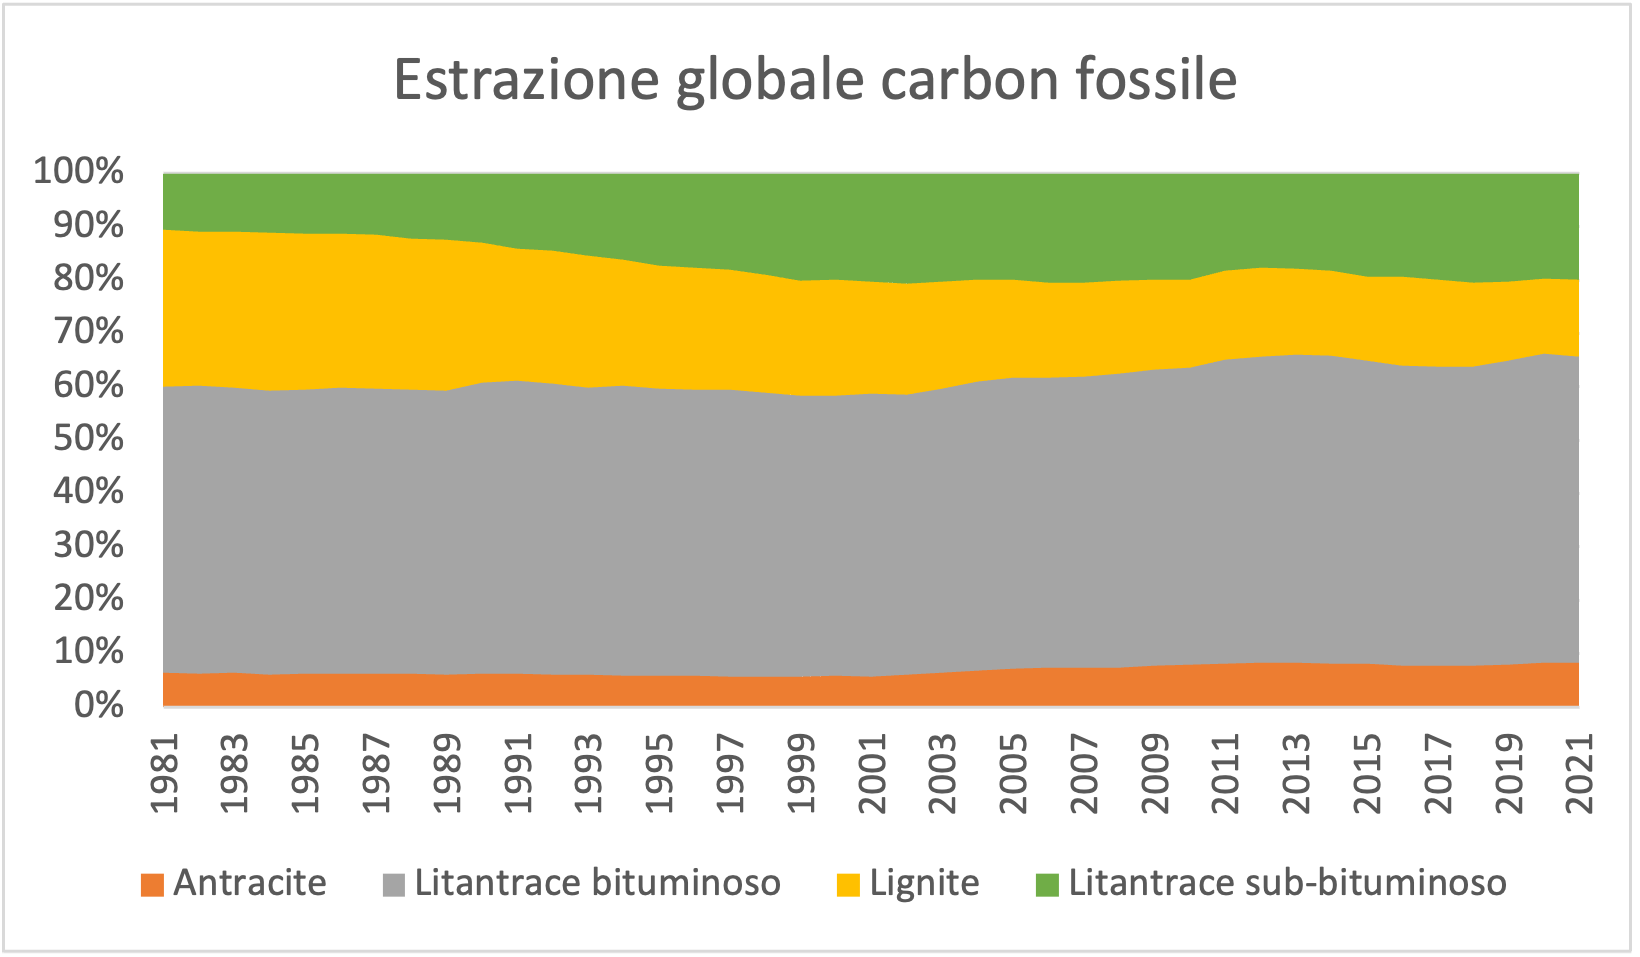
\includegraphics[height=0.6\textwidth]{res/cap 2/Grafico carbone}
    \caption{Grafico rappresentate la quantità di carbone estratta globalmente negli ultimi 40 anni}
\end{figure}\noindent
Prenderemo quindi il litantrace bituminoso il quale è il più largamente estratto e consumato, risulta che abbia la seguente composizione in peso:\cite{Composizione-antracite}\\
\begin{itemize}
    \item Carbonio(84.4\%)
    \item Ossigeno(6.7\%)
    \item Idrogeno(5.4\%)
    \item Azoto(1.7\%)
    \item Zolfo(1.8\%)
\end{itemize}
Si noti come in questo caso vi è un contenuto anche di altre sostante, oltre ad idrogeno e carbonio, tra le quali si evidenzia lo zolfo la cui presenza porta a dei residui di combustione altamente impattanti a livello ambientale.\\
Data la formazione chimica più complessa andare a portare una grossa semplificazione, come fatto in precedenza, riporterebbe un dato totalmente falsato e poco significativo; per questo motivo sarà riportato il valore contenuto in alcune tabelle che si attesta attorno ai  $20\frac{KJ}{Kg}$ valore che spesso, data la formazione chimica del carbone che può variare di molto da giacimento a giacimento, viene calcolato sperimentalemente.\\
Il prezzo riportato in questo caso è in $\frac{\$}{short ton}$ una \enquote{short ton} equivale a 2000lb quindi a circa 907kg, tenendo conto del potere calorifero riportato in precedenza si arriva ad un valore finale di circa $0,01\frac{\$}{MJ}$.
\vfill
\newpage
\subsection{Petrolio}
Il petrolio, una volta estratto, deve subire diverse lavorazioni prima di poter venir usato per produrre energia. Il processo che porta il petrolio ad essere frazionato è quello della distillazione.\\
La lavorazione del petrolio si compone di molteplici fasi le quali avvengono in sequenza sui diversi componenti estratti per andare a sfruttare al massimo la materia prima.\\
La componente che per questa sezione verrà presa in considerazione è quella degli oli combustibili. Questi sono oli pesanti utilizzati prevalentemente per la produzione di energia in centrali termoelettriche e per il settore navale sempre come combustibile.
Anche in questo caso il problema dell'utilizzo di queste sostanze come combustibile è l'alto tenore di zolfo che contengono. Esso, una volta avvenuta la combustione, andrà a combinarsi con l'ossigeno e l'idrogeno contenuti in atmosfera andando a generare acido solforico e acido nitrico provocando i fenomeni comunemente chiamati piogge acide.\\
Da un barile di petrolio\footnote{42 galloni statunitensi $\sim$159 litri} si ricavano circa 45 galloni di prodotti raffinanti con la suddivisione indicata nella tabella sottostante\cite{composizione-petrolio}:\\
\begin{table}[!ht]
    \centering
    \begin{tabular}{|l|l|l|}
    \hline
        \textbf{Prodotto} & \textbf{Quantità[gal]} & \textbf{\%} \\ \hline
        Finished motor gasoline & 20,08 & 45,07\% \\ \hline
        Distillate fuel oil & 12,47 & 27,99\% \\ \hline
        Kerosene-type jet fuel & 3,53 & 7,92\% \\ \hline
        Petroleum coke & 2,06 & 4,62\% \\ \hline
        Still gas & 1,72 & 3,86\% \\ \hline
        Hydrocarbon gas liquids & 1,68 & 3,77\% \\ \hline
        Asphalt and road oil & 0,92 & 2,07\% \\ \hline
        Residual fuel oil & 0,59 & 1,32\% \\ \hline
        Naptha for feedstocks & 0,46 & 1,03\% \\ \hline
        Lubricants & 0,46 & 1,03\% \\ \hline
        Other oils for feedstocks & 0,25 & 0,56\% \\ \hline
        Miscellaneous products & 0,21 & 0,47\% \\ \hline
        Special napthas & 0,08 & 0,18\% \\ \hline
        Finished aviation gasoline & 0,04 & 0,09\% \\ \hline
        \textbf{TOTALE} & \textbf{44,55} & \\ \hline
    \end{tabular}
\end{table}\\
Per ogni barile di petrolio grezzo al termine del processo di raffinazione si ottengono 0,59 galloni di olio combustibile che è il prodotto che ci interessa per questa sezione.
Facendo riferimento a dati tabulati troviamo che il potere calorifico dell'olio combustibile è di $41,022 \frac{MJ}{kg}/$, dopo le opportune conversioni, otteniamo un valore di $0,00017\frac{\$}{MJ}$.
Non sono neanche in questo caso stati inseriti i costi di estrazione, trasporto e successiva raffinazione in quanto altamente variabili e difficilmente stimabili.
    %!TEX root = ../main.tex

\chapter{Impianti}
\label{chp:impianti}
Nel capitolo precedente sono state elencate e brevemente introdotte le varie fonti energetiche che abbiamo a disposizione. Sarà obbiettivo di questo capitolo elencare ed illustrare il funzionamento degli impianti utilizzabili per convertire le varie fonti energetiche in energia elettrica la quale sarà poi immessa nella rete elettrica.\\
\section{Impianto fotovoltaico}
Un impianto fotovoltaico è un impianto elettrico formato da più moduli fotovoltaici i quali, sfruttando l'energia solare, producono energia elettrica mediante il così detto l'effetto fotovoltaico.\\
All'interno di un impianto fotovoltaico possiamo identificare alcuni elementi chiave e fondamentali come:
\begin{itemize}
    \item Cavi, diodi e magnetotermici
    \item Inverter
\end{itemize}
I primi sono fondamentali per la connessione e la sicurezza dell'impianto mentre i secondi sono necessari per la conversione DC-AC per poi poter immettere in rete l'energia elettrica che si produce.\\
Per illustrare il funzionamento di un impianto è importante prima capire il funzionamento dell'effetto fotovoltaico.\\
\subsection{Effetto fotovoltaico}
Durante lo studio delle onde elettromagnetiche si notò come una radiazione elettromagnetica che investe un materiale possa, in certe condizioni, cedere energia agli elettroni più esterni degli atomi del materiale stesso. Se l'energia risulta sufficiente l'elettrone è libero di staccarsi dall'atomo di origine ed allontanarsi.\\
Questo fenomeno però non può essere sfruttato in tutti i materiali. Negli isolanti, per esempio, il gap tra la banda di condizione e la banda di valenza, chiamato band gap, è troppo elevato per poter essere eguagliato dall'energia del fotone incidente. Per i materiali conduttori, invece, vi è una continua creazione e distruzione di coppie elettrone-lacune e l'energia necessaria per la creazione di esse viene fornita direttamente dalla variazione di temperatura.\\
Al contrario, quando un fascio luminoso investe un semiconduttore si verifica il passaggio in banda di conduzione di un certo numero di elettroni al quale corrisponde un uguale numero di lacune che passa in banda di valenza.\\
Per generare un flusso di elettroni è necessario creare un campo elettrico all'interno della cella, per tale scopo si sfrutta il drogaggio. Il drogaggio consiste nell'inserire atomi diversi dal silicio all'interno di alcune zone del semiconduttore per ottenere due zone: la prima con eccesso di lacune(zona p) la seconda con eccesso di elettroni(zona n).\\
\begin{figure}[H]
    \centering
    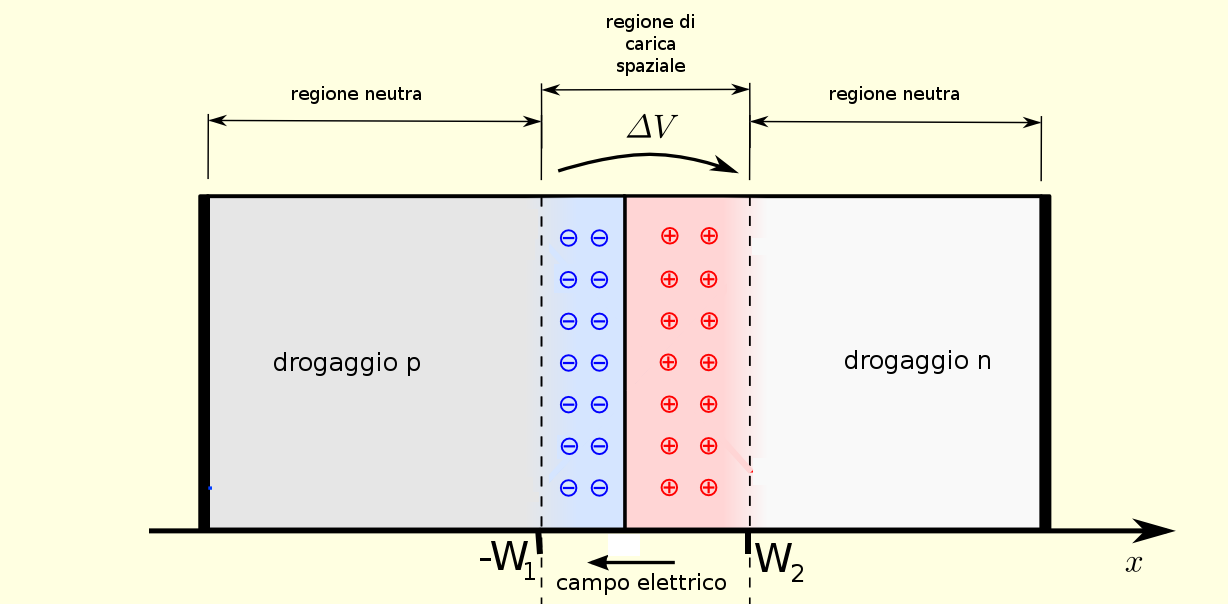
\includegraphics[height=0.5\textwidth]{res/cap 3/drogaggio}
    \caption{Rappresentazione di semiconduttore con drogaggio p-n}
\end{figure}\noindent
Si formano quindi due zone, la prima con una prevalenza di elettroni liberi e la seconda con lacune le quali provocano una carenza di elettroni andandosi a creare un campo elettrico che si estende a cavallo della regione di svuotamento.
Grazie al fenomeno illustrato in precedenza se si illumina la giunzione dalla parte n vengono a crearsi delle copie elettrone-lacune in entrambe le zone, il campo elettrico presente a causa del drogaggio fa si che gli elettroni in eccesso si dividano e li spinge in direzioni opposte. Una volta oltrepassata la regione di svuotamento non possono quindi più tornare indietro a causa della presenza del campo elettrico.\\
Procedendo quindi con una connessione esterna si otterrà un circuito chiuso nel quale il flusso di elettroni parte dallo strato n,a potenziale maggiore, per dirigersi nello strato p, a potenziale minore fintanto che la cella rimanere esposta ai raggi solari.\\
\subsection{Cella solare}
Una cella solare è un dispositivo elettrico a stato solido il quale tramite l'effetto fotovoltaico permette di convertire l'energia trasportata dalla luce solare in elettricità tramite l'effetto illustrato nella sezione precedente.\\
La maggior parte delle celle fotovoltaiche prodotte, se esposte al sole, producono una tensione di circa 0.6V, è quindi necessario metterle in serie per ottenere tensioni più alte.
Collegando le celle in serie però non si ha il controllo sulle singole celle in quanto la stessa corrente attraversa tutte le celle, quelle poste in ombra quindi finiscono per fare da strozzatura per tutto il sistema andando a scaldarsi e potenzialmente a danneggiarsi.\\
E' quindi visibile l'importanza di posizionare correttamente i pannelli fotovoltaici in modo che vi siano delle zone d'ombra e per meno periodi possibili.\\
\subsection{Pannello fotovoltaico}
\paragraph{Struttura}\mbox{}\\
Un pannello fotovoltaico è formato da un'insieme di celle opportunamente collegate tramite una griglia metallica che è presente sulla superficie del modulo in modo da formare sia collegamenti in serie che in parallelo. Una volta collegate le celle si procede con l'assemblaggio del modulo ponendo sopra la superficie posteriore, realizzata con un materiale isolante con scarsa dilatazione termica, uno strato di acetato di vinile(EVA), si pone quindi lo strato di celle solare opportunamente collegate per poi porre un'ulteriore strato di EVA ed il vetro temperato a protezione dell'intero modulo.\\
\begin{figure}[H]
    \centering
    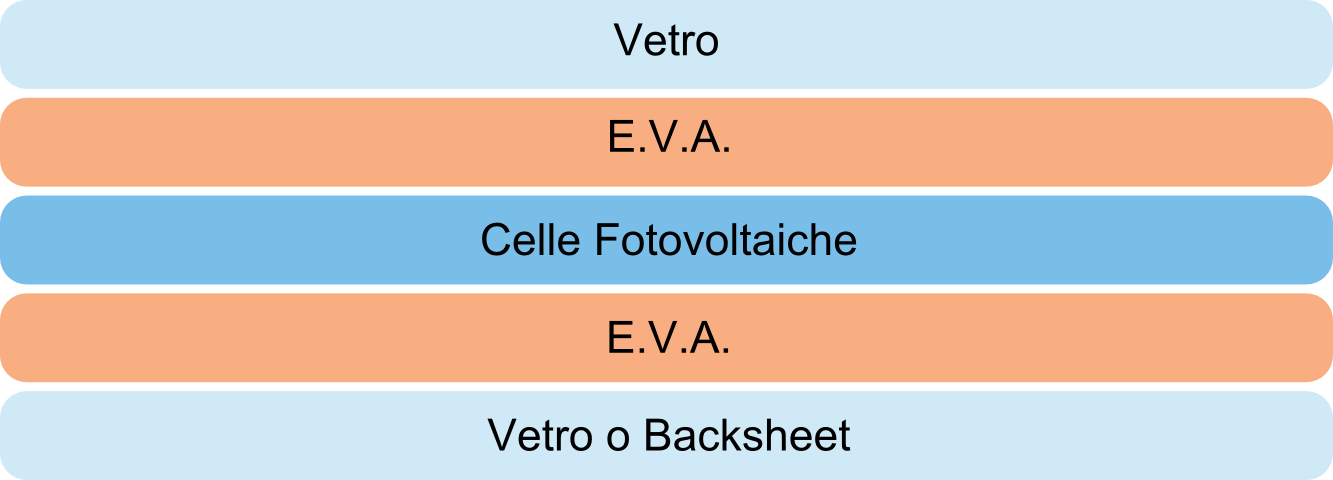
\includegraphics[height=0.3\textwidth]{res/cap 3/composizione modulo}
    \caption{Schema di composizione di un modulo fotovoltaico}
\end{figure}\noindent
Una volta assemblato si procede con un processo di pressofusione atto a trasformare l'EVA in un collante inerte, si collega la griglia ad una morsettiera che viene posta sul retro e si chiude il modulo in un frame di alluminio che faciliterà l'installazione e l'orientamento.
\paragraph{Tecnologie realizzative}\mbox{}\\
Dei molti semiconduttori utilizzabili per la produzione dei moduli fotovoltaici il più comunemente usato è il silicio, esso si ottiene in wafer che successivamente vengono uniti tra loro a formare un modulo.\\
Esistono diverse tipologie costruttive delle celle, tra le più comuni troviamo:
\begin{description}[labelindent=5mm]
    \item[$\cdot$ Silicio monocristallino:] ogni cella è realizzata a partire da un wafer formato da un monocristallo opportunamente drogato. Sono tendenzialmente costose in quanto risulta difficile formare ampie superfici senza sprecare materiale o spazio, però permettono di raggiungere un'efficienza dell'ordine del 18-21\%.
    \item[$\cdot$ Silicio policristallino:] in questo caso la cella è formata da un policristallo, quindi non strutturalmente omogeneo ma organizzato in grani localmente ordinati. Il costo in questo caso data la peggior qualità del silicio usato risulta più basso a favora di una maggior facilità di taglio e lavorazione. L'efficienza raggiungibile con questa tipologia di silicio però è più bassa del caso precedente e si attesta nell'ordine del 15-17\%. 
    \item[$\cdot$ Silicio amorfo:] questa tipologia di celle hanno un'efficienza più bassa ($\sim8\%$) ma risultano molto più economici da produrre rispetto ad i precedenti. Il silicio amorfo ha un bandgap più ambio dei precedenti(circa un 55\% in più) il che favorisce l'assorbimento della parte visibile dello spettro solare ma risulta meno efficiente nell'elaborare la parte infrarossa.
\end{description}
\paragraph{Prestazioni ed efficienza}\mbox{}\\
Le prestazioni offerte dal singolo modulo dipendono da diversi fattori, in prima fase, si può calcolare, in modo approssimato, la potenza che un pannello è in grado di esprimere con la seguente formula:
\begin{center}
    \large{$P = \eta I_0 S \sin(\alpha)  $}
\end{center}
Dove con $I_0$ si considera l'irradianza perpendicolare alla superficie, con S la superficie del modulo, mentre $\alpha$ è l'angolo che il modulo ha con il sole, $\eta$ invece è un fattore di rendimento.\\
In conclusione possiamo osservare come i parametri fisici che influenzano la produzione di un pannello solare possano essere sintetizzati in:
\begin{itemize}
    \item Irraggiamento a cui il pannello è esposto
    \item Angolo con la quale in modulo è orientato
    \item Qualità produttiva del modulo
    \item Tipologia di silicio usato
\end{itemize}
Si nota anche qui l'importanza di collocare il pannello in una regione che abbiamo una buona copertura da parte del sole ed in una superficie correttamente orientata.\\
Nel caso di installazioni su tetti questi due parametri rendono o meno un determinato tetto idoneo all'installazione, nel caso si installino in campi fotovoltaici invece l'angolo di installazione viene scelto in fase costruttiva quindi ideale per il luogo in cui è collocato.\\
Come visto in precedenza l'angolo con cui la luce solare colpisce la terra dipende sia dal luogo geografico che dal periodo dell'anno preso in esame, vi sarà quindi un'efficienza diversa da periodo data dall'inclinazione del modulo oltre che dalle condizioni climatiche.\\
Il singolo modulo in condizioni normali lavora in un range di tensione a vuoto($V_{OC}$) tra 40 ed i 50 Volt ed una corrente di cortocircuito($I_{sc}$) tra i 9 ed i 12 Ampere.\\
Un altro fattore importante che influenza negativamente il rendimento di un pannello fotovoltaico è la temperatura, infatti la temperatura della giunzione p-n va ad influenzare sia ($V_{OC}$) che ($I_{sc}$) andando quindi ad alterare anche la potenza massima($P_{Max}$) che il modulo è in grado di offrire.\\
Per quantificare l'impatto della temperatura sul pannello ogni produttore fornisce tre valori tre espressi in $\frac{\%}{^\circ C}$:
\begin{enumerate}
    \item Coefficiente di temperatura di ($P_{Max}$)
    \item Coefficiente di temperatura di ($V_{OC}$)
    \item Coefficiente di temperatura di ($I_{sc}$)
\end{enumerate}
\newpage
\section{Impianto eolico}
Un impianto eolico è un sistema che converte l'energia del vento in energia elettrica.
Gli elementi fondamentali che lo compongono sono:
\begin{description}[labelindent=5mm]
    \item[$\bullet$ Pale eoliche]: sono le parti rotanti che catturano l'energia del vento, deve essere possibile variarne l'angolo di calettamento per ottimizzarne il funzionamento.
    \item[$\bullet$ Moltiplicatore di giri]: consente di prendere in input un certo numero di giri ad una determinata coppia e dare in output un numero superiore di giri ad una coppia più bassa.
    \item[$\bullet$ Generatore eolico]: è un dispositivo che converte l'energia meccanica generata dalla rotazione delle pale in energia elettrica.
    \item[$\bullet$ Torre eolica]: sostiene le pale ed il generatore permettendone l'installazione ad un'altezza adeguata per catturare il vento in maniera adeguata.
    \item[$\bullet$ Elettronica di controllo] controlla il funzionamento complessivo dell'impianto con lo scopo di mantenere alte performance e standard di sicurezza elevati.
\item \end{description}
A questi elementi principali che compongono un impianto eolico si possono aggiungere, a seconda delle dimensioni e delle esigenze, altri componenti come inverter, sistemi di raffreddamento.
Saranno ora brevemente illustrati i vari componenti e ne sarà spiegato in modo sintetico il funzionamento e principi che li guidano.
Una prima suddivisione va fatta in base alle forma, infatti esistono fondamentalmente due tipi di turbine:
\begin{itemize}
    \item \textbf{HAWT} (Horizontal Axis Wind Turbines)
    \item \textbf{VAWT} (Vertical Axis Wind Turbines)
\end{itemize}
Le prime possono essere configurate sia con rotore sopravvento che sottovento, nel primo caso si ha il vantaggio di non avere interferenza di alcun tipo da parte della torre mentre nel secondo caso la macchina è in grado di orientarsi in automatico.
Nel caso di turbine VAMT,invece, vi è la caratteristica di essere immuni alla direzione del vento ma tendenzialmente avere una resa rispetto allo spazio occupato inferiore rispetto al caso precedente.
\subsection{Caratteristiche e casi d'uso HAWT e VAWT}
\paragraph{HAWT}\mbox{}\\
Le caratteristiche principali di una turbina eolica a elica orizzontale (HAWT) sono le seguenti:
\begin{description}[labelindent=5mm]
    \item[$\bullet$ Alta efficienza]: Le turbine HAWT sono progettate per catturare l'energia del vento in modo efficiente, con rendimenti più elevati rispetto alle turbine VAWT.
    \item[$\bullet$ Adatte ai venti forti]: Le turbine HAWT sono particolarmente adatte ai venti forti, poiché la loro progettazione a elica orizzontale le rende in grado di catturare l'energia del vento in modo più efficiente.
    \item[$\bullet$ Dimensioni maggiori]: Le turbine HAWT sono generalmente più grandi delle turbine VAWT, il che le rende adatte per l'installazione in aree con spazi più ampi.
    \item[$\bullet$ Funzionamento più rumoroso]: Le turbine HAWT possono essere più rumorose delle turbine VAWT, poiché l'elica che gira rapidamente è più vicina alla superficie terrestre.
\end{description}
Date le caratteristiche peculiari di questa tipologia di turbine alcuni casi d'applicazione possono essere:
\begin{description}[labelindent=5mm]
    \item[$\bullet$ Impianti di grandi dimensioni]: Le turbine HAWT sono adatte per la costruzione di impianti di grandi dimensioni, infatti possono produrre grandi quantità di energia elettrica.
    \item[$\bullet$ Parchi eolici]: Le turbine HAWT sono spesso utilizzate per la costruzione di parchi eolici, dove vengono installate molte turbine per produrre energia elettrica a livello commerciale.
    \item[$\bullet$ Installazioni offshore]: Le turbine HAWT possono essere installate in mare per sfruttare i venti più forti che soffiano al largo della costa.
    \item[$\bullet$ Alimentazione elettrica per grandi comunità]: Le turbine HAWT possono essere utilizzate per fornire energia elettrica a grandi comunità, come città e fabbriche.
\end{description}
Le turbine di tipologia HAWT sono l'unica opzione percorribile quando lo scopo dell'installazione è generare grandi quantità di energia in presenza di venti di intensità sostenuta.
Tuttavia essendo particolarmente rumorose e visivamente impattanti la loro installazione è spesso effettuata offshore o a distanza dalle comunità.
\begin{figure}[H]
    \centering
    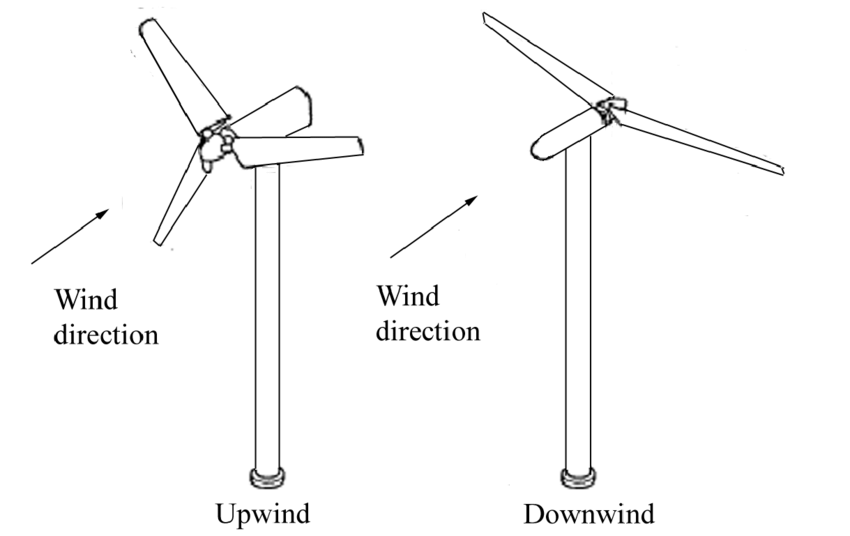
\includegraphics[height=0.3\textwidth]{res/cap 3/HAWT}
    \caption{Esempio di turbina HAWT sopravvento e sottovento}
\end{figure}\noindent
\paragraph{VAWT}\mbox{}\\
Le caratteristiche principali di una turbina eolica ad elica verticale (VAWT) sono le seguenti:
\begin{description}[labelindent=5mm]
    \item[$\bullet$ Design compatto]: Le pale sono disposte verticalmente, il che le rende più compatte e adatte per l'installazione in aree limitate.
    \item[$\bullet$ Funzionamento silenzioso]: Sono progettate per funzionare in modo più silenzioso rispetto alle pale HAWT (a elica orizzontale), poiché non vi è un'elica che gira rapidamente nella vicinanza della superficie terrestre generando quindi meno rumore.
    \item[$\bullet$ Minor influenza dal vento irregolare]: Sono meno influenzate dal vento irregolare rispetto alle pale HAWT, poiché il loro design a elica verticale le rende più stabili e meno sensibili alle perturbazioni del vento.
    \item[$\bullet$ Adatte per venti deboli]: Sono particolarmente adatte per i venti deboli, poiché possono catturare energia dai venti deboli che soffiano in direzioni diverse rispetto alle pale HAWT che necessitano di venti di direzione costante e di intensità più sostenuta.
\end{description}
Date le caratteristiche appena descritte i casi specifici di applicazione che si possono identificare sono i seguenti:
\begin{description}[labelindent=5mm]
    \item[$\bullet$ Piccole comunità rurali]: Le turbine VAWT possono essere utilizzate per fornire energia elettrica a piccole comunità rurali che altrimenti non sarebbero in grado di accedere ai servizi di energia elettrica.
    \item[$\bullet$ Sistemi di energia solare ibridi]: Le turbine VAWT possono essere utilizzate insieme a sistemi di energia solare per fornire un'alimentazione elettrica affidabile durante tutto l'anno.
    \item[$\bullet$ Edifici residenziali e commerciali]: Le turbine VAWT possono essere utilizzate per fornire energia elettrica a edifici residenziali e commerciali, riducendo la loro dipendenza dalla rete elettrica nazionale.
    \item[$\bullet$ Sistemi di energia marini]: Le turbine VAWT possono essere utilizzate per fornire energia elettrica a sistemi di energia marini, come piattaforme petrolifere e rig.
\end{description}
Le turbine di tipologia VAWT sono un'opzione valida per fornire energia elettrica in tutte quelle situazioni in cui sono necessarie turbine compatte, silenziose e adatte ai venti deboli.
Tuttavia, il loro rendimento è generalmente inferiore rispetto alle pale HAWT, quindi potrebbero non essere la scelta migliore per grandi campi eolici.
\begin{figure}[H]
    \centering
    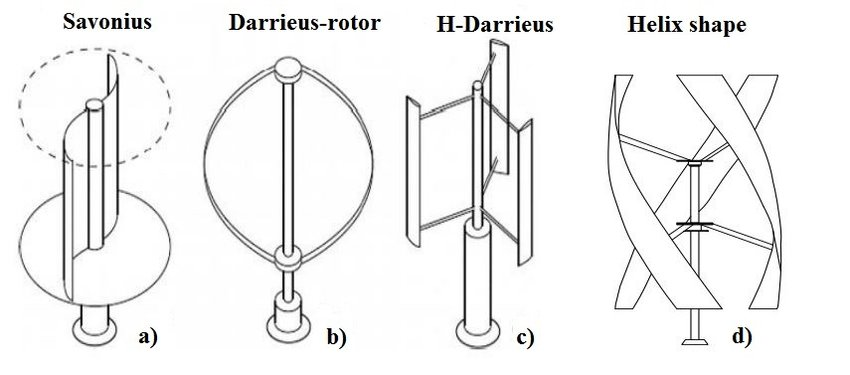
\includegraphics[height=0.3\textwidth]{res/cap 3/VAWT}
    \caption{Esempio di diverse tipologie di turbine VAWT}
\end{figure}\noindent
\subsection{Prestazioni ed efficienza}
Per descrivere questo capitolo è importante parlare e specificare il limite di betz in quanto pone il limite superiore di efficienza raggiungibile da qualsiasi impianto eolico.\\
Il limite di Betz porta a descrivere il rendimento come segue è espresso come segue:\\
\large{$\eta = \frac{16}{27} \cdot (1 - (\frac{v_2}{v_1})^2)$}\\
dove:\\
\large{$\eta$} è il coefficiente di prestazione (rendimento) della turbina eolica\\
\large{$v_1$} è la velocità del vento all'ingresso della turbina\\
\large{$v_2$} è la velocità del vento all'uscita della turbina.\\
Il limite di Betz rappresenta il massimo rendimento teorico che può essere ottenuto da una turbina eolica corrisponde a un coefficiente di prestazione pari a $\frac{16}{27}$ pari a circa il 60\%.\\
Nella pratica, le turbine eoliche reali hanno rendimenti molto più bassi, solitamente compresi tra il 20\% e il 50\% a causa di fattori come la resistenza dell'aria, la turbolenza e la frizione all'interno della turbina. Tuttavia, il limite di Betz fornisce un punto di riferimento importante per la valutazione dell'efficienza delle turbine eoliche.
\paragraph{HAWT}\mbox{}\\
Le prestazioni e l'efficienza delle turbine eoliche a elica orizzontale (HAWT) sono determinate da una serie di fattori, tra cui la velocità del vento, la densità dell'aria, la geometria della turbina e la tecnologia utilizzata.
L'efficienza delle turbine HAWT può essere valutata utilizzando il coefficiente di prestazione, che rappresenta la quantità di energia catturata dalla turbina rispetto all'energia del vento disponibile.\\
In generale, come visto sopra, le turbine HAWT hanno coefficienti di prestazione compresi tra il 40\% e il 50\%.\\
La velocità del vento è un fattore critico per le prestazioni delle turbine HAWT. A velocità del vento maggiori, la turbina produce più energia elettrica. Tuttavia, se la velocità del vento supera un certo limite, la turbina può essere danneggiata o subire un arresto di sicurezza.\\
La tecnologia utilizzata nelle turbine HAWT influisce anche sulle prestazioni. Ad esempio, l'utilizzo di materiali leggeri e resistenti come la fibra di carbonio può aumentare la durata e la resistenza delle pale della turbina, migliorando le prestazioni a fronte però di un sostanzioso aumento dei costi costruttivi.\\
Inoltre, l'utilizzo di sistemi di controllo avanzati può aiutare a ottimizzare la produzione di energia elettrica in base alle condizioni del vento andando ad esempio a far variare l'angolo di attacco delle pale in modo da adattarlo alla velocità del vento presente ottimizzando i flussi.
\paragraph{VAWT}\mbox{}\\
Le turbine VAWT hanno alcune caratteristiche uniche che le rendono adatte a determinate situazioni e poco adatte per altre per questo motivo si utilizzano, non per cercare una grande efficienza, ma quando il caso specifico lo richiede.
In termini di prestazioni, le turbine VAWT hanno una efficienza inferiore rispetto alle turbine HAWT, la quale si attesta generalmente intorno al 30-40\%.
Si nota come questo range sia inferiore rispetto a quello riscontrato nelle turbine HAWT però compensato dalla possibilità di essere inserite in contesti particolari e di richiedere mediamente meno manutenzione e garantendo una maggior semplicità di installazione non dovendo ad esempio essere orientate.
\newpage
\section{Centrale a biomasse}
La tipologia di impianti che sfruttano la digestione anaerobica per produrre biogas il quale andrà ad alimentare una caldaia.\\
Parlando di impianti a digestione anaerobica è importante descrivere le fasi che la compongono:\\
\begin{description}[labelindent=5mm]
    \item[$\bullet$ Produzione di acidi grassi]: i batteri scompongono gli zuccheri, amidi e grassi presenti nella biomassa in acidi grassi, come l'acido solfidrico e l'acido lattico.
    \item[$\bullet$ Fermentazione]: gli acidi grassi vengono ulteriormente decomposti da altri batteri anaerobici in biossido di carbonio (CO2) e metano (CH4). Questo processo è chiamato fermentazione acida o acidogenesi.
    \item[$\bullet$ Maturazione]: durante questa fase, i resti della digestione anaerobica vengono trasformati in compost stabile da batteri aerobi. Questo compost può essere utilizzato come fertilizzante per la coltivazione di piante.
\end{description}
Questi processi avvengono appunto all'interno di un digestore dal quale si avrà in output il biogas ed il substrato digerito il quale sarà ricco di sostanze quali: azoto, fosforo, potassio.
La quantità di biogas che si è in grado di estrarre dipende da diversi fattori quali:
\begin{description}[labelindent=5mm]
    \item[$\bullet$ Composizione chimica della biomassa]: la quantità di biogas prodotta dipende dalla quantità e dalla qualità dei componenti presenti nella biomassa, come ad esempio zuccheri, amidi, proteine e grassi.
    \item[$\bullet$ Condizioni ambientali]: il pH, la temperatura ed il tempo di digestione.
    \item[$\bullet$ Tipo di batteri]: il tipo di batteri utilizzati e dalla loro capacità di decomporre la biomassa in biogas.
    \item[$\bullet$ Dimensione e tecnologia dell'impianto]: vi è una dipende anche dalla capacità dell'impianto e dalla tecnologia utilizzata per la digestione anaerobica(presenza di sistemi di miscelazione o di controllo di processo).
\end{description}
Il processo necessita quindi della presenza di batteri i quali andranno a decomporre la sostanza organica, vi sono 3 tipo di batteri diversi i quali operano a diverse temperature ed hanno tempi di permanenza nel reattore diversi:\\
\begin{description}[labelindent=5mm]
    \item[$\bullet$ Batteri psicrofili]: sono batteri che si sviluppano a temperature comprese tra 5°C e 25°C. Sono adatti a processi che avvengono a temperature più basse.La loro permanenza nel sistema di digestione è di circa 10-12 settimane.
    \item[$\bullet$ Batteri mesofili]: sono batteri che si sviluppano a temperature comprese tra 25°C e 45°C. Sono adatti a processi che avvengono a temperature medie e la loro permanenza è di circa 3-8 settimane.
    \item[$\bullet$ Batteri termofili]: sono batteri che si sviluppano a temperature comprese tra 45°C e 60°C. Sono adatti a processi che avvengono a temperature elevate e la loro permanenza è di circa 2-3 settimane.
\end{description}
La scelta del tipo di batteri da utilizzare dipende quindi,in generale, dalle condizioni ambientali e dal tipo di biomassa che si desidera trattare.La selezione dei batteri più adatti aumenta l'efficienza e la quantità di biogas prodotto durante la digestione anaerobica.\\
\begin{figure}[H]
    \centering
    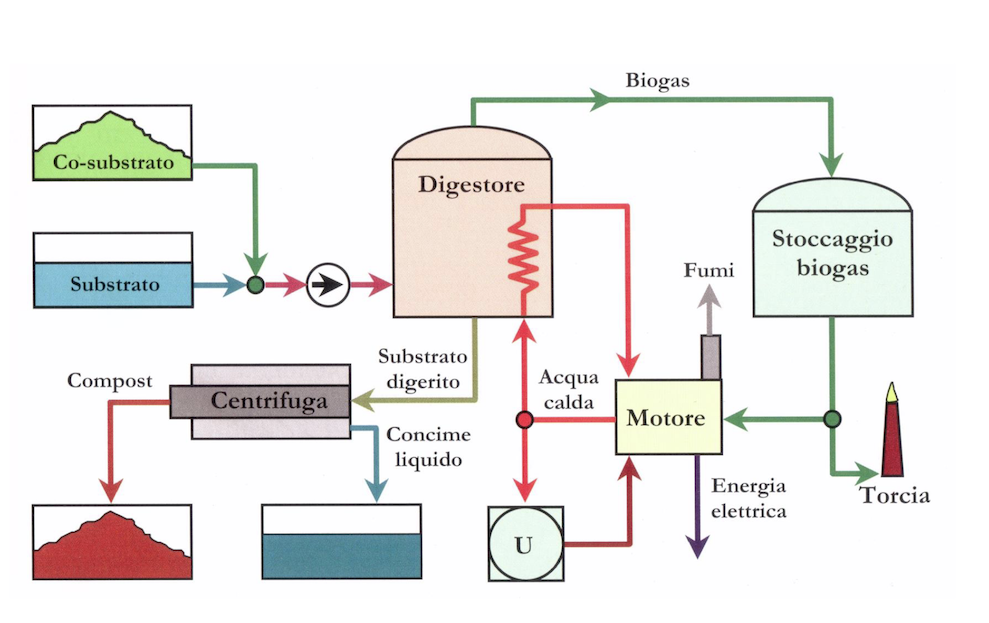
\includegraphics[height=0.5\textwidth]{res/cap 3/Biomasse}
    \caption{Esempio di uno schema di un'impianto a biomasse con digestore anaerobico\cite{Materiale_didattico_prof_savino}}
\end{figure}\noindent
\section{Impianti per correnti marine}
Questa tipologia di impianti sfrutta l'energia cinetica delle correnti marine per produrre energia elettrica.\\
Vengono utilizzate turbine a elica simili a quelle utilizzate nei generatori eolici per trasformare l'energia cinetica dell'acqua in energia meccanica, che viene poi convertita in energia elettrica attraverso l'utilizzo di generatori elettrici.\\
Le turbine a elica possono essere sia collocate su una struttura galleggiante che su una fissa fissa la quale è comunque ancorata al fondale marino.
La produzione di energia è direttamente proporzionale alla velocità della corrente e alla superficie della turbina da qui l'importanza di effettuare una corretta scelta di posizionamento e dimensionamento dell'impianto, scelta che influenza poi alcune scelte costruttive e strutturali.
Esistono infatti due tipi principali di turbine ad elica utilizzate negli impianti a energia delle correnti marine: le turbine ad asse orizzontale e le turbine ad asse verticale.\\
Le turbine ad asse orizzontale, simili a quelle utilizzate nei generatori eolici, hanno le pale dell'elica montate su un asse orizzontale che ruota intorno ad un mozzo centrale.\\
Le turbine ad asse verticale, invece, hanno le pale dell'elica montate su un asse verticale che ruota intorno a un mozzo centrale.\\
\begin{figure}[H]
    \centering
    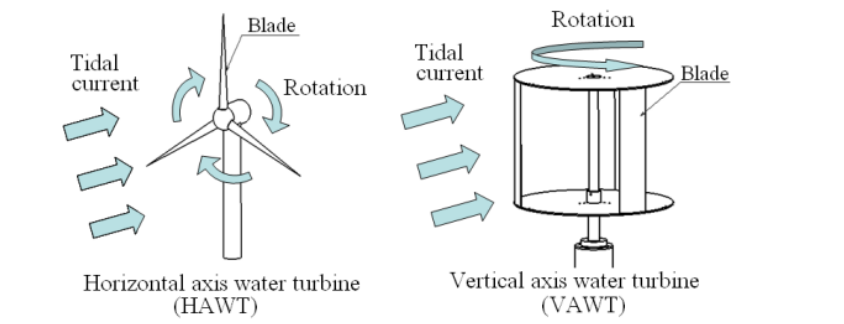
\includegraphics[height=0.4\textwidth]{res/cap 3/Ocean current turbine}
    \caption{Esempio di varie tipologie di turbine ad asse vericale\cite{Ocean_current_turbine}}
\end{figure}\noindent
La scelta della tipologia di turbina da utilizzare dipende quindi dalle condizioni dell'ambiente in cui l'impianto viene installato:Le turbine ad asse orizzontale, ad esempio, sono più adatte per acque poco profonde e correnti con una direzione del flusso costante, mentre le turbine ad asse verticale sono più adatte per acque più profonde e correnti con una direzione del flusso variabile.\\
Gli impianti che sfruttano l'energia delle correnti marine presentano alcuni vantaggi rispetto ad altre tecnologie di produzione di energia rinnovabile: in particolare, le correnti marine sono costanti e prevedibili, il che significa che la produzione di energia è più affidabile e continua rispetto ad altre fonti di energia rinnovabile.
Inoltre non interferiscono con le attività di pesca o la navigazione che possono avvenire in totale normalità a patto che l'impianto sia stato correttamente progettato e posizionato.\\
Di contro gli impianti a energia delle correnti marine possono avere anche un impatto negativo sull'ambiente marino e sulla vita marina se la loro struttura non è costruita in modo da impedire contatti accidentali con le parti in movimento.\\
\section{Centrali mareomotrici}
Le centrali mareomotrici sono tutta quella tipologia di impianti che sfruttano l'energia mareomotrice che si ricava dallo spostamento dell'acqua causato dalle maree.\\
Si possono identificare quattro tipologia di impianti che sfruttano l'energia delle maree ma il funzionamento finale è molto simile per tutti:\\
\begin{itemize}
    \item Sollevamento di un peso
    \item Compressione dell'acqua in opportuni cassoni e movimentazione delle turbine in espansione
    \item Mobimento di ruote a pale(più usato nell'antichità che in epoca moderna)
    \item Riempimento di bacini e successivo svuotamento con passaggio(sia in ingresso che in uscita) attraverso turbine
\end{itemize}
Sarà illustrato il funzionamento degli impianti a bacino in quanto sono i maggiormente usati per sfruttare questa tipologia di fenomeno.\\
\subsection{Impianti a bacino}
In questa tipologia di impianto, l'energia delle maree viene utilizzata per riempire un bacino artificiale durante l'alta marea.Nel canale che permette all'acqua di entrare nel bacino sarà presente una turbina la quale sarà in grado di lavorare sia durante la fase di \enquote{carico} che durante la fase di \enquote{scarico} dal bacino.\\
In termini di efficenza ovviamente la turbina sarà progettata per essere ottimizzata per una delle due direzioni dell'acqua.Una scelta alternativa potrebbe essere quella di collocare due due turbine orientate in verso opposto in modo da avere il massimo rendimento in entrambe le fasi con un ovvio e conseguente aumento di costo dell'impianto.\\
Il funzionamento della centrale a riempimento di bacino inizia con la costruzione di una diga o di uno sbarramento che blocca l'ingresso di acqua salata in un'area costiera o in un'estuario.
Il processo avviene in due fasi collegate allo stato della marea: fase di carico e fase di scarico.\\
La prima avviene durante la fase di alta marea momento in cui all'acqua salata viene permesso di entrare nel bacino fino a riempirlo.Questo processo avviene durante la fase di massima marea per poter sfruttare al massimo l'altezza piezometrica disponibile.\\
La seconda invece avviene durante la fase di bassa marea, momento nel quale l'acqua contenuta nel bacino si trova ad un livello superiore a quella del mare esterno.\\
Infatti durante la bassa marea, la diga viene aperta e l'acqua del bacino viene fatta fluire attraverso turbine situate alla base della diga.
L'energia cinetica dell'acqua fa girare le turbine, che alimentano un generatore elettrico per produrre energia elettrica.
Il vantaggio di questa tipologia di impianti è il poter sempre prevedere quando ed in che modo il bacino sarà riempito e quindi prevederne la produzione elettrica, di contro spesso si possono riscontrare le maree sfalsate rispetto alla reale necessità di energia.\\
Per ovviare a questo problema si potrebbe inserire un ulteriore bacino discarico che funzioni un po' da pre-camera e tramite un sistema di paratoie andare ad ottimizzare la fase di scarico per sovrapporla a quella di maggior consumo elettrico.\\
La stessa tipologia di impianto e con il medesimo funzionamento può anche essere collocato alla foce di un fiume, come avviene in francia a Saint-Malo, in questo caso l'impatto visivo è sicuramente minore non dovendo costruire ex-novo dei bacini artificiali sulla zona costiera.\\
\begin{figure}[H]
    \centering
    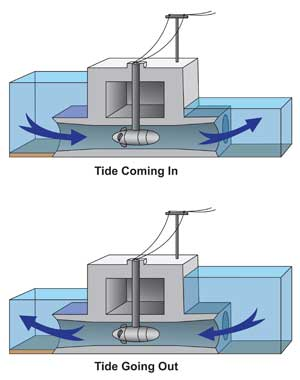
\includegraphics[height=0.35\textwidth]{res/cap 3/Tidal-power-300}
    \caption{Schema esemplificativo di impianto a bacino}
\end{figure}\noindent
\paragraph{Impatto ambientale}\mbox{}\\
L'impatto ambientale considerato sia nella fase di costruzione che nella fase di operatività dell'impianto, nella prima è richiesta la realizzazione di dighe o sbarramenti per creare bacini artificiali per l'accumulo di acqua.
Ciò può portare a una variazione dell'habitat marino e dell'ecosistema locale.Inoltre, la costruzione dell'impianto richiede la movimentazione di grandi quantità di terra e la costruzione di strutture portanti, che possono danneggiare o distruggere habitat naturali importanti.\\
Durante la fase di esercizio invece le centrali possono influenzare la salinità e la temperatura dell'acqua in mare aperto e nelle zone costiere.L'acqua che viene rilasciata dal bacino artificiale può avere una temperatura e una salinità diverse rispetto all'acqua circostante, il che può influire sulla flora e fauna marina locale.Inoltre, le turbine e le altre componenti meccaniche dell'impianto possono rappresentare un rischio per la fauna marina, come i mammiferi marini o i pesci migratori, che possono rimanere intrappolati o feriti.\\
\section{Impianti idroelettrici}
In questa sezione sono inseriti tutta quella tipologia di impianti i quali sfruttano l'energia dell'acqua in un punto nella fase del ciclo dalla sorgente al mare.\\
In un'impianto si possono identificare due bacini: uno di monte, uno di valle ed una condotta che li collega che può essere a pelo libero od in pressione.In un punto intermedio tra i due bacini sarà collocata la centrale idroelettrica nella quale avverrà la conversione dell'energia cinetica dell'acqua in energia elettrica.\\
Questa tipologia di impianti sfrutta quindi l'energia potenziale del bacino di monte la quale perdendo quota acquisirà energia cinetica che andrà poi elaborata all'interno della centrale dalla turbina.\\
\begin{figure}[H]
    \centering
    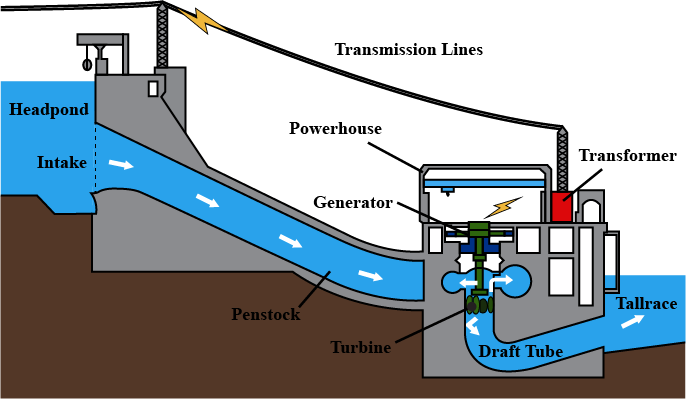
\includegraphics[height=0.4\textwidth]{res/cap 3/hpp diagram}
    \caption{Schema di una centrale idroelettrica}
\end{figure}\noindent
Sono presenti tre tipologie principali di turbine che andranno scelte in base al contesto specifico:
\begin{itemize}
    \item Pelton
    \item Francis
    \item Kaplan
\end{itemize}
\vfill
\newpage
\begin{figure}[H]
    \centering
    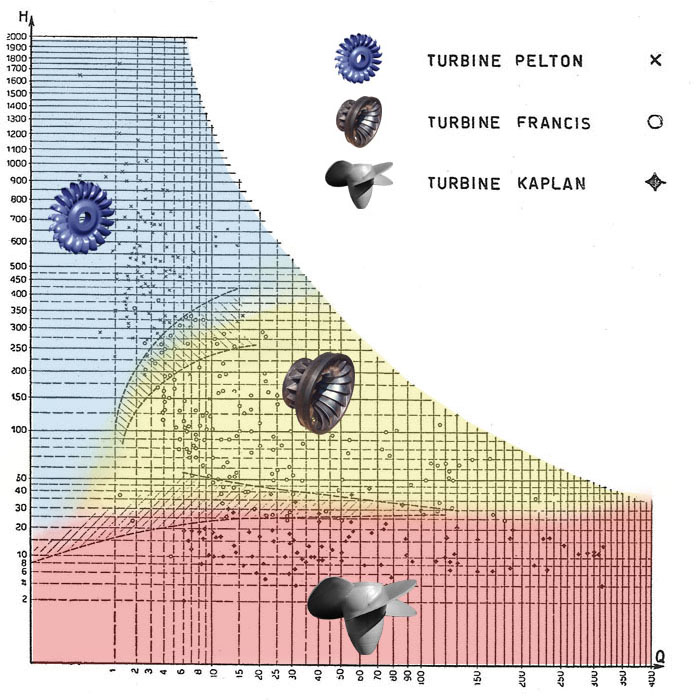
\includegraphics[height=0.4\textwidth]{res/cap 3/1_Campi-applicazione}
    \caption{Schema illustrativo dei campi di applicazione delle tre tipologie}
\end{figure}\noindent
Come è possibile vedere le turbine pelton sono in grado di elaborare una piccola portata ma un grande salto, le francis si posizionano invece con caratteristiche intermedie tra le due mentre le kaplan sono in grado di elaborare grandi portate ma con un salto contenuto.\\
Prima di illustrare singolarmente le caratteristiche delle tre tipologie è importante descrivere il funzionamento del Tubo aspiratore diffusore(TAD),un componente di fondamentale importante per le ultime due in quando permette un grande recupero di energia che altrimenti andrebbe dispersa.
\subsection{Tubo aspiratore diffusore}
Il TAD è un condotto che ha il compito di collegare lo scarico della turbina con il bacino di valle:
\begin{figure}[H]
    \centering
    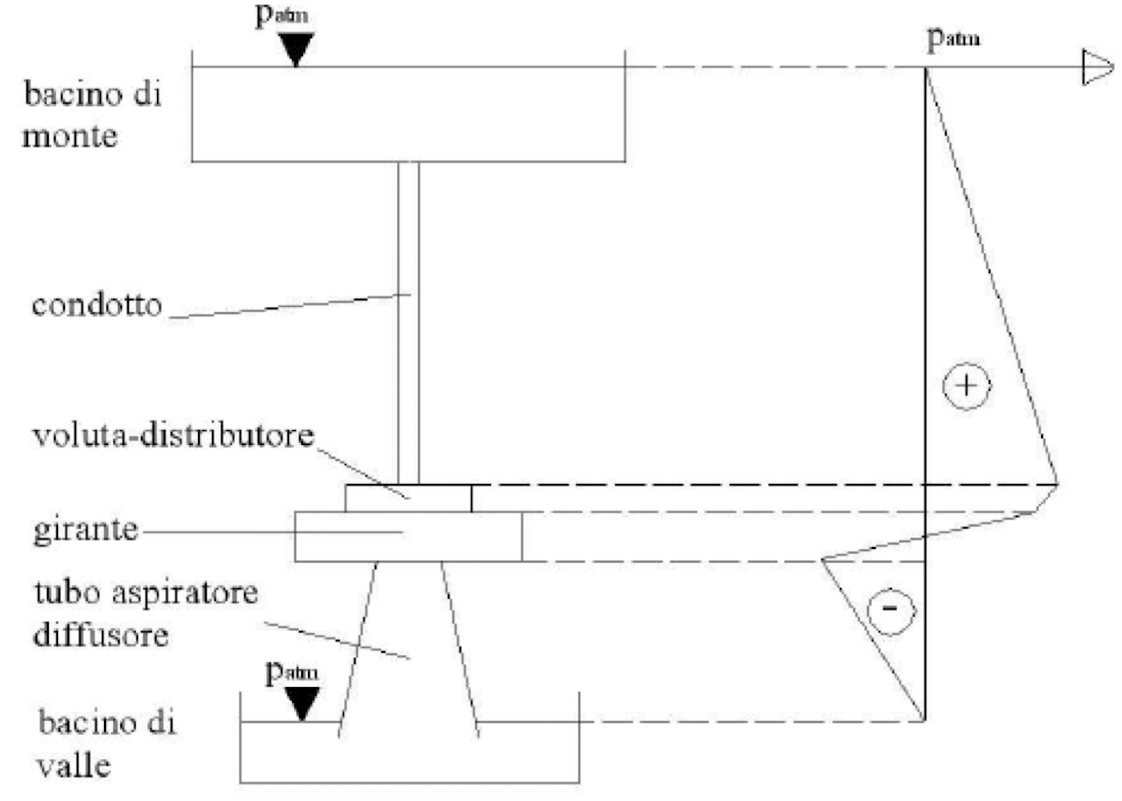
\includegraphics[height=0.4\textwidth]{res/cap 3/francis con TAD}
    \caption{Importanta del TAD}
\end{figure}\noindent
Questo componente infatti permette il recupero di parte dell'energia cinetica e del salto a valle ed di fondamentale importanza nelle turbine Francis e Kaplan.\\
Per spiegarne il funzionamento vengono illustrati tre scenari che si possono configurare a valle:
\begin{enumerate}
    \item Scarico a pressione atmosferica senza condotta
    \item Scarico con condotta a sezione costante
    \item Scarico con condotta a sezione variabile(TAD)
\end{enumerate}
Nel primo caso salto a valle ed energia cinetica vengono persi, installando un tubo a sezione costante si riesce a a recuperare il salto a valle ma non l'energia cinetica mentre le terzo caso è possibile recuperare entrambe.
Applicando il teorema di bernoulli:
\begin{center}
    \large{$p_1+\frac{1}{2}\rho v_1^2 + \rho g h_1 = p_2+\frac{1}{2}\rho v_2^2 + \rho g h_2$}
\end{center}
La densità del fluido rimane costante, mentre \large{$p_2$} corrisponde alla pressione atmosferica, possiamo poi indicare la velocità come rapporto tra la portata e la sezione.
\begin{center}
    \large{$p_1+\frac{1}{2}\rho \frac{Q}{s_1}^2 + \rho g h_1 = p_{atm}+\frac{1}{2}\rho \frac{Q}{s_2}^2 + \rho g h_2$}
\end{center}
Nel caso quindi di un tubo a sezione costante il secondo termine da entrambe le parti può essere semplificato in quando non varia trovandosi con la seguente relazione:
\begin{center}
    \large{$p_1 + \rho g h_1 = p_{atm}+ \rho g h_2$}
\end{center}
La pressione in uscita dalla turbina risulta quindi:
\begin{center}
    \large{$p_1 = p_{atm} + \rho g (h_2 - h_1)$}
\end{center}
Essendo la quota di scarico inferiore alla quota di aspirazione ci si trova ad avenre una pressione \large{$p_1<p_{atm}$} elaborando quindi parte dell'energia che sarebbe altrimenti andata persa.\\
Aggiungendo invece una sezione variabile ci si trova a non avere il secondo elemento costante:
\begin{center}
    \large{$p_1 = p_{atm} + \frac{1}{2}\rho Q^2 (\frac{1}{s_2^2} - \frac{1}{s_1^2}) + \rho g (h_2 - h_1)$}
\end{center}
In questo caso anche il secondo fattore sarà negativo in quanto il TAD ha una sezione in ingresso più piccola di quella in uscita, si ottiene quindi un'ulteriore recupero di salto piezometrico.\\
Le caratteristiche geometriche di questo condotto vanno attentamente studiate in quando un'errata progettazione potrebbe portare ad un fenomeno chiamato cavitazione.
Il fluido allo scarico della turbina trovandosi in uno stato di bassissima pressione si trova a cambiare di stato trasformandosi in vapore e subendo un grande aumento di volume.
Il vapore avendo un volume maggiore dell'acqua genera un'aumento della velocità del fluido, ma una volta tornato ad una pressione che lo riporta in uno stato liquido può generare onde di pressione che rischiano di danneggiare i componenti meccanici
\vfill
\subsection{Pelton}
Questa tipologia, come precedentemente spiegato, è in grado di elaborare un grande salto(400-1800 m) ma portate medio piccole(1-10$\frac{m^3}{s}$), ottenendo quindi un range di potenza indicativo di 100-300MW.\\
E' una turbina ad azione($\varepsilon=0$), ciò indica che il salto piezometrico che il fluido mette a disposizione è elaborato solamente dall'organo distributore.
\begin{figure}[H]
    \centering
    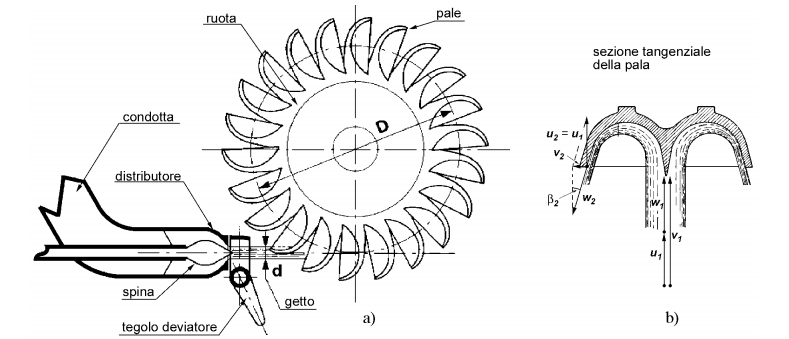
\includegraphics[height=0.4\textwidth]{res/cap 3/pelton}
    \caption{Schema di comprendente gli elementi principali di una turbina pelton}
\end{figure}\noindent
In questa tipologia di turbine dovendo operare con salti notevoli l'acqua arriva all'interno di una condotta forzata, il flusso poi viene deviato e raggiunge il/gli ugello/i la cui numerosità è definita dalla portata dell'acqua.
Una volta raggiunti gli ugelli la \enquote{spina doble} permette di convertire la pressione del fluido in energia cinetica indirizzando un getto direttamente sui cucchiai della girante la quale ruotando trasmette energia meccanica all'alternatore.\\
Il rendimento massimo ottenibile da questa tipologia di turbina nel caso ideale si ottiene quando ci si trova ad avere un rapporto $\frac{u}{c_1}=0.5$ dove c1 rappresenta la velocità dell'acqua e u rappresenta la velocità periferica della ruota.
Noti i parametri di portata e caduta è quindi opportuno progettare la macchina perchè rispetti quel rapporto:\\
\begin{enumerate}
    \item Conoscendo la portata Q posso definire diversi parametri:\\
        \begin{center}
            \large{$Q=\frac{\pi}{4}\cdot d^2 \cdot c_1 \cdot i$}
        \end{center}
        Con d il diametro del getto, \large{$c_1$} la velocità in uscita del getto ed i il numero degli iniettori
    \item Ricavati d e \large{$c_1$} voglio che la macchina lavori ad \large{$\eta$} massimo che si ottine con un rapporto \large{$\frac{u}{c_1}=0.5$} noto \large{$c_1$} posso ricavare u e trammite la legge \large{$u=\omega r$} posso ricavare il raggio della girante
\end{enumerate}
Per il progetto della geometria della turbina sono invece ben definire le geometrie degli angoli delle pale.
\subsection{Francis}
Questa tipologia di turbina è quella tra le tre più polivalente, è in grado infatti di elaborare portate in un range molto ampio(4-150$\frac{m^3}{s}$) ma anche salti notevoli(40-400m),queste caratteristiche le permettono un'ampio spettro di applicazione con potenze che anche in questo caso oscillano tra i 100 ed i 300MW.\\
A differenza della precedente la francis è una turbina a reazione($\varepsilon>0$) il che significa che in questo caso anche la girante contribuisce ad elaborare il salto piezometrico.
\begin{figure}[H]
    \centering
    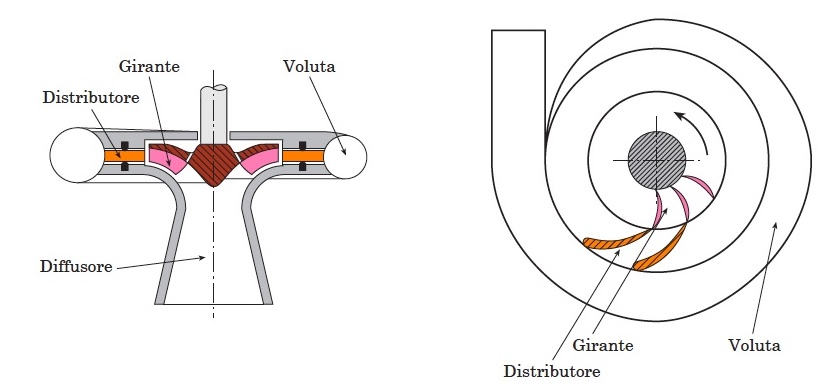
\includegraphics[height=0.4\textwidth]{res/cap 3/francis}
    \caption{Schema di una turbina francis}
\end{figure}\noindent
In questo caso l'acqua inizia a scorrere all'interno della voluta la quale ha appositamente una sezione variabile in modo da poter mantenere costante la velocità del fluido al suo interno.
L'acqua a questo punto attraversa il distributore il quale ha una serie di pale orientabili le quali hanno lo scopo di elaborare la prima parte del salto piezometrico convertendo parte della pressione del fluido in velocità, è fondamentale che le pale siano orientabili in quanto permettono la regolazione della macchina.\\
La girante in questo caso ha la caratteristica che ricevere il fluido radialmente e di scaricarlo assialmente convertendo l'energia cinetica dell'acqua in energia meccanica.
Di fondamentale importanza allo scarico è l'inserimento di un TAD per permettere una miglior efficienza.\\
Per quanto riguarda la fase progettuale ci si basa sulle caratteristiche di turbine già esistenti e funzionanti, si conosce infatti la portata(Q) il salto piezometrico(H) e il numero di giri a cui la macchina debba operare(n) e da esse tramite diagrammi specifici si possono ricavare tutti i parametri dimensionali.
\newpage
\subsection{Ad elica o Kaplan}
Questa tipologia di turbina permette di elaborare portate elevate(>100\large$\frac{m^3}{s}$) però con salti contenuti(<90m), queste caratteristiche la collocano in'ambito d'utilizzo molto specifico raggiungendo però solitamente potenze inferiori a quelle delle altre turbine(<200MW).\\
Anche in questo caso ci troviamo davanti ad una turbina a reazione con un Kq solitamente superiore alle francis.
La differenza sostanziale tra le turbine ad elica e le kaplan sta nel fatto che le seconde possono far variare il calettamento delle pale rotoriche oltre che quello delle pale del diffusore, permettendo di raggiungere il massimo grado di efficienza in condizioni diverse.
\begin{figure}[H]
    \centering
    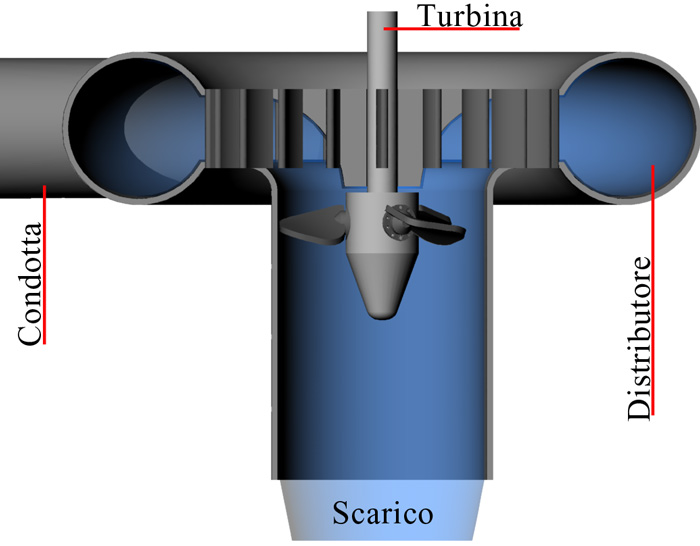
\includegraphics[height=0.4\textwidth]{res/cap 3/kaplan}
    \caption{Schema di una turbina kaplan}
\end{figure}\noindent
Anche in questo caso a livello progettuale si parte dal fatto che si conoscano i principali parametri quali portata, salto e numero di giri della turbina(Q,H,n) e da li tramite una serie di tabelle caratteristiche si calcolano i parametri dimensionali della macchina.
    %!TEX root = ../main.tex

\chapter{Photovoltaic Geographical Information System(PGIS)}
\label{chp:Photovoltaic Geographical Information System(PGIS)}

\section{Introduzione al tool(PVGIS)}
Il tool in questione è sviluppato e reso disponibile a titolo gratuito dal \enquote{Joint Research Centre}; Fornice un'interfaccia user friendly per accedere ad un database contenente dati sull'irradianza in differenti locazioni geografiche e permette di calcolare grafici di produzione o di esportare dati specifici sulle condizioni meteo di una determinata zona.\\
E' possibile accedere al \href{https://re.jrc.ec.europa.eu/pvg_tools/it/}{\underline{PVGIS tool}} trovandosi a lavorare con quest'interfaccia:\\
\begin{figure}[H]
    \centering
    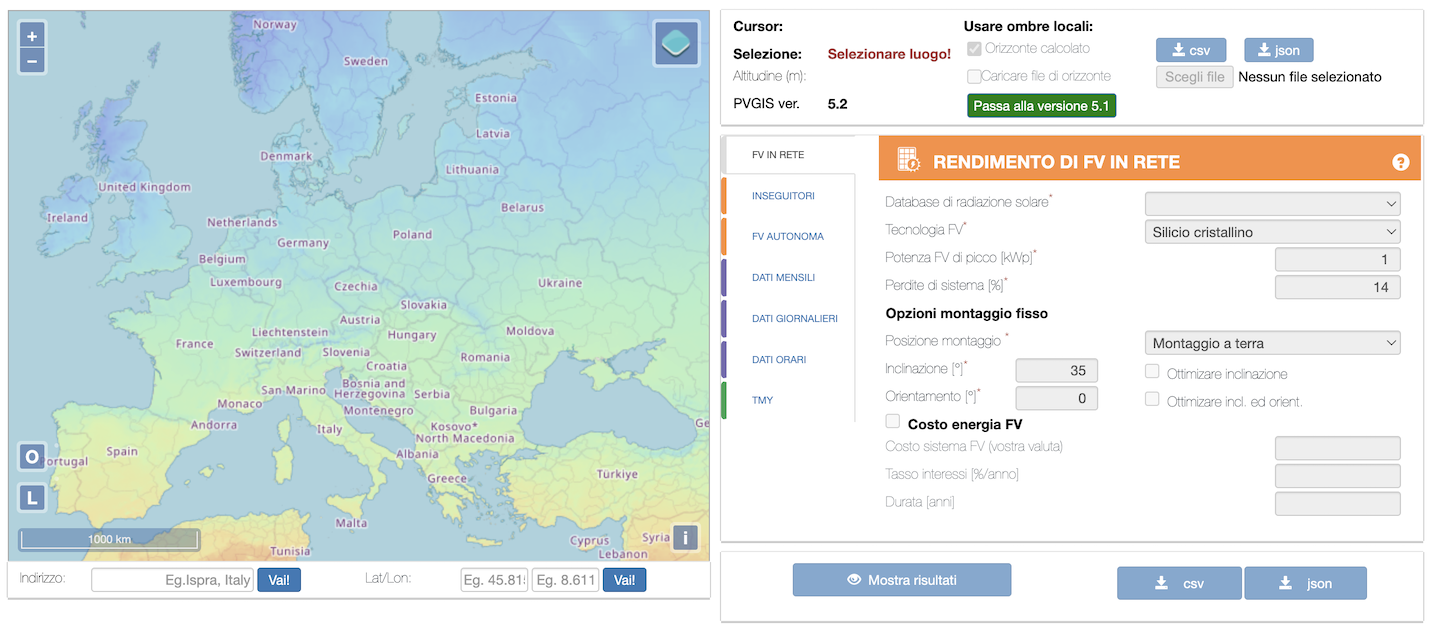
\includegraphics[height=0.5\textwidth]{res/cap 4/PGIS_schermata principale}
    \caption{Interfaccia PVGIS}
\end{figure}\noindent
La prima scelta che va fatta per iniziare ad usar il tool è quella di scegliere una locazione, in questo esempio verrà utilizzata come posizione quella del polo scientifico dell'università di udine(46.081, 13.212).\\
Si procederà poi scegliendo se inserire un file contenente i dati dell'orizzonte o se procedere con un calcolo automatico di esso.
Il primo caso risulta molto comodo quando vi sono ostruzioni naturali od artificiali che possono generare ombra nella superficie che si vuole analizzare.\\
Nel caso si voglia procedere con l'inserimento manuale il programma richiede di inserire una serie di valori, uno per ogni riga, rappresentanti l'altezza dell'orizzonte, misurati in gradi dall'orizzontale.
Le altezze nel file sono considerate ordinante in senso orario partendo da nord, se per esempio si inseriscono quindi 10 valori il programma considera una misurazione ogni $37^\circ$.\\
Una volta operata l'importante scelta riguardo all'orizzonte si può procedere con l'utilizzo del tool.\\
Lo strumento permette di calcolare diverse applicazioni del fotovoltaico e di estrarre diversi parametri meteorologici con cadenza mensile settimanale o giornaliera.
Nel menù laterale possiamo quindi scegliere se di effettuare 3 tipologie di calcoli su ambiti applicativi diversi:
\begin{itemize}
    \item Fotovoltaico in rete
    \item Fotovoltaico ad inseguimento in rete
    \item Fotovoltaico con accumulo
\end{itemize}
Sarà presentata ora una sintetica descrizione delle varie opzioni percorribili
\subsection{Fotovoltaico in rete}
\begin{figure}[H]
    \centering
    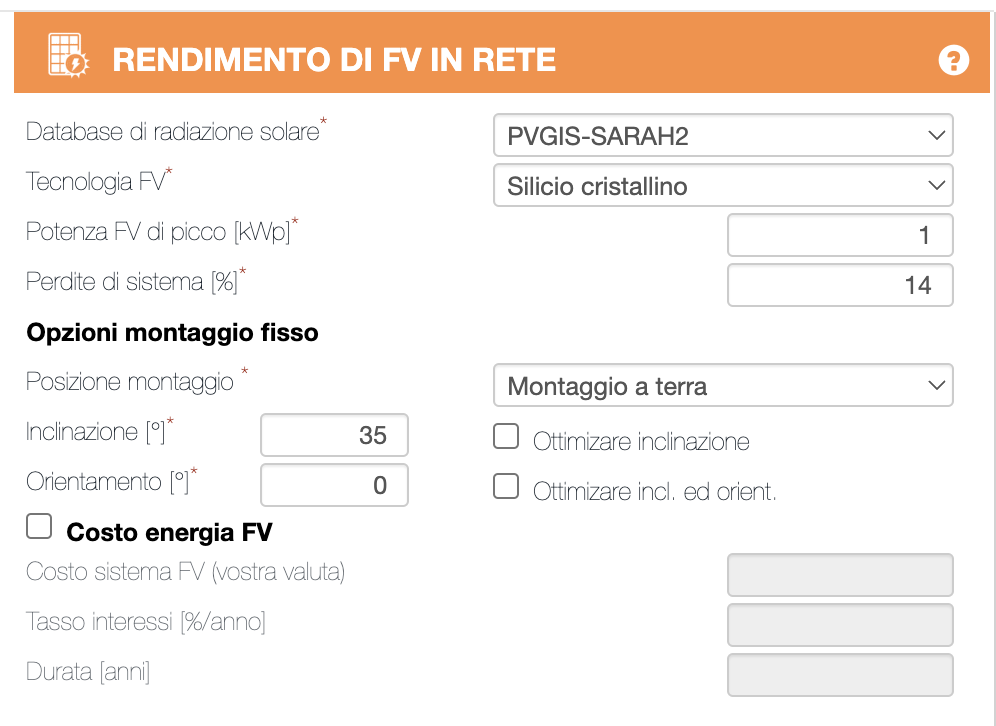
\includegraphics[height=0.5\textwidth]{res/cap 4/Fotovoltaico statico}
    \caption{Scheda fotovoltaico in rete}
\end{figure}\noindent
Come visibile nel'immagine superiore è necessario specificare al sistema diversi parametri quali:
\begin{description}[labelindent=5mm]
    \item[$\bullet$ Database di radiazione solare]: sono proposti tre tipologie di database diversi che si differenziano per range dei dati presenti e per risoluzione che per tutti è inferiore agli \large{$0.5^{\circ}$}
    \item[$\bullet$ Tecnologia fotovoltaico]: sono presenti sia pannelli classici definiti a silicio cristallino che 2 tipologie di moduli a film sottili
    \item[$\bullet$ Potenza di picco]: è la potenza che un modulo è in grado di esprimere ricevendo \large{$1000\frac{W}{m^2}$} perpendicolarmente ad una temperatura di \large{$25^{\circ}C$},è un valore comunque espresso nella scheda tecnica dei moduli fotovoltaici
    \item[$\bullet$ Perdite di sistema]: rappresenta un valore percentuale che esprire tutte le perdire che vanno a ridurre la quantità di energia resa alla rete elettrica, sono incluse in questo valore: perdite resistive dei cavi, perdite dovute all'efficienza dell'inverter, presenza di sporco sui moduli, invecchiamento dei moduli stessi. Il software consiglia automaticamento l'uso di un valore medio di 14\%.
\end{description}
Sono poi da inserire tutte quelle caratteristiche che riguardano l'installazione dell'impianto e sono spesso decise a priori nel caso in cui l'installazione avvenga su un tetto.
\begin{description}[labelindent=5mm]
    \item[$\bullet$ Posizione di montaggio]: i sistema permette di selezionare un montaggio libero, oppure un montaggio su un tetto di un'edificio, nel secondo caso il pannello(a parità di inclinazione) rende meno rispetto al corrispettivo a terra a causa di un minor rendimento dovuto alla temperatura.
    \item[$\bullet$ Inclinazione]: si intende l'angolo che avrà il modulo rispetto all'orizzontale, è possibile lasciare al software il compito di scegliere in autonomia l'inclinazione nel caso non sia un parametro già fissato da fattori fisici
    \item[$\bullet$ Orientamento]: è l'angolo che il modulo avrà rispetto a sud con valori positivi verso ovest e negativi verso est, anche in questo caso l'angolo può essere calcolato in automatico dal software
\end{description}
\vfill
\subsection{Fotovoltaico ad inseguimento in rete}
\begin{figure}[H]
    \centering
    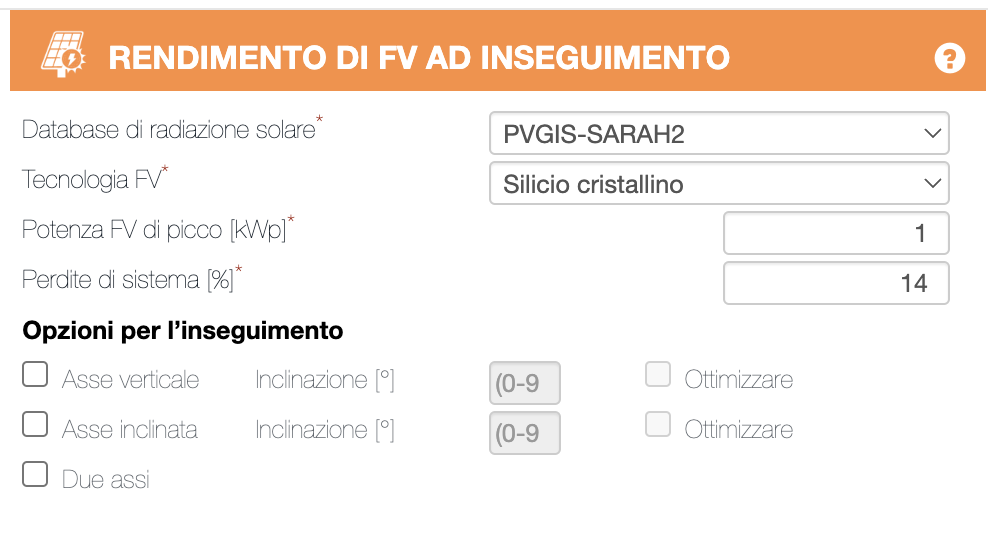
\includegraphics[height=0.5\textwidth]{res/cap 4/moduli ad inseguimento}
    \caption{Scheda fotovoltaico in rete ad inseguimento}
\end{figure}\noindent
Alcuni parametri rimangono identici a quelli illustrati nel caso precedente, a questi si aggiungono:
\begin{description}[labelindent=5mm]
    \item[$\bullet$ Asse verticale]: i moduli sono montati su una struttura con asse di rotazione verticale, l'asse orizzontale è fisso, il suo valore può essere inserito manualmente o calcolato automaticamente.
    \item[$\bullet$ Asse inclinata]: i moduli sono montati su una struttura mobile con un'asse di rotazione inclinata orientata in direzione nord-sud, i moduli vanno montati in modo parallelo all'asse di rotazione, l'inclinazione può essere inserita manualmente o calcolata automaticamente.
    \item[$\bullet$ Due assi]: i moduli sono montati in una struttura mobile su entrambi gli assi quindi risultano totalmente ad inseguimento.
\end{description}
\vfill
\subsection{Fotovoltaico con accumulo}
\begin{figure}[H]
    \centering
    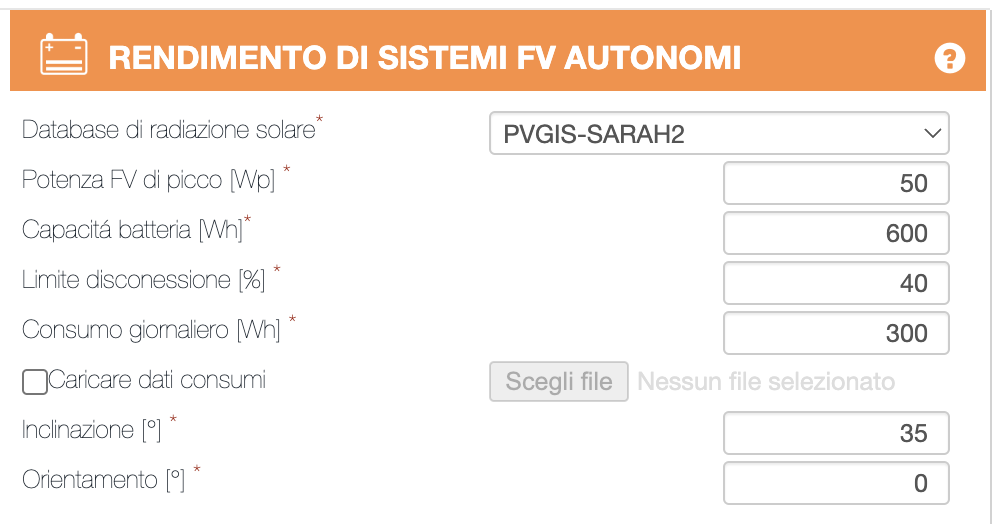
\includegraphics[height=0.5\textwidth]{res/cap 4/fotovoltaico con accumulo}
    \caption{Scheda fotovoltaico con accumulo}
\end{figure}\noindent
In questo caso la scheda risulta diversa dalla precedente in quanto, oltre a tanti parametri trovati nella prima scheda, sono presenti diversi parametri legati alla capacità del stoccaggio disponibile ed al consumo dell'abitazione:
\begin{description}[labelindent=5mm]
    \item[$\bullet$ Capacità batteria]: capacità grezza delle batterie, considerando di poterle scaricare all 100\%
    \item[$\bullet$ Limite di disconnessione]: limite inferire al quale si può scaricare la batteria per evitare di danneggiarla,strettamente legato alla tecnologia della batteria, le batterie al litio ad esempio possono subire una scarica più profonda senza subire danni
    \item[$\bullet$ Consumo giornaliero]: consumo elettrico in un periodo di 24 ore, il software per dividerlo nelle varie ore del giorno utilizza un profilo basato su dati statistici
\end{description}
E' possibile inoltre specificare manualmente il proprio profilo di consumo per rendere i dati più veritieri per il proprio uso
\subsection{Export dati mensile}
\begin{figure}[H]
    \centering
    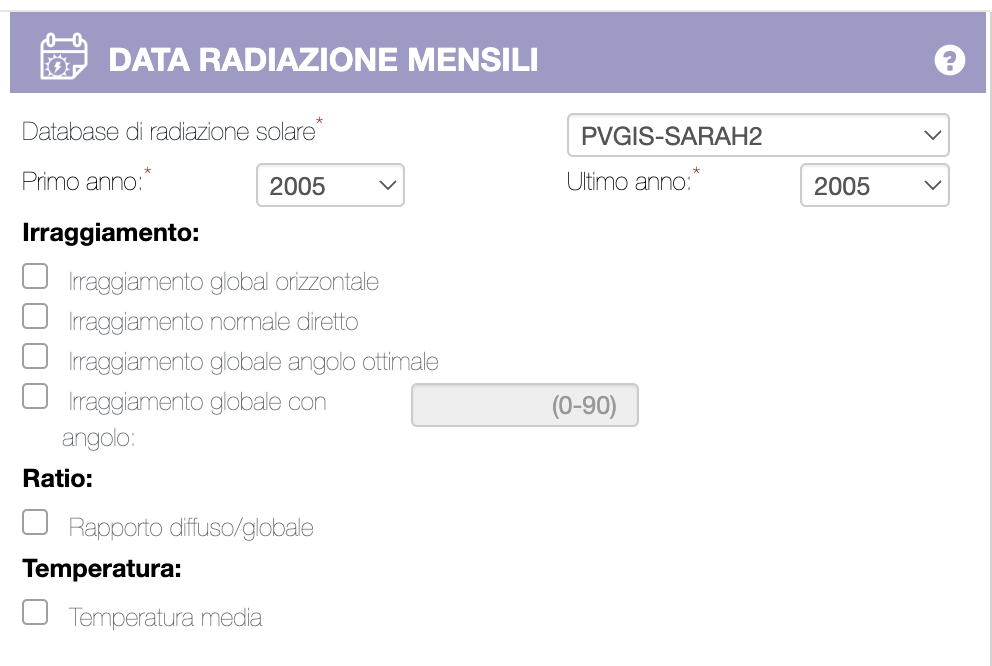
\includegraphics[height=0.5\textwidth]{res/cap 4/dati mensili}
    \caption{Scheda dati mensili}
    \label{fig:export mensile}
\end{figure}\noindent
Tramite questa scheda una volta selezionato l'orizzonte temporaneo da prendere in analisi, il range disponibile dipende dal modello scelto, per quello presente in'immagine ad esempio sono presenti dati dal 2005 al 2020.
L'export può comprendere tutti i dati in figura:
\begin{description}[labelindent=5mm]
    \item[$\bullet$ Irraggiamento globale orizzontale]: rappresenta la somma mensile dell'energia delle radiazioni su ogni metro quadro di piano orizzontale
    \item[$\bullet$ Irraggiamento normale diretto]: rappresenta la somma mensile dell'energia delle radiazione su un piano che segue il sole in modo da puntarlo sempre direttamente, include le sole radiazioni provenienti direttamente dal sole e non quelle che arrivano per altri fenomeni.
    \item[$\bullet$ Irraggiamento globale con angolo ottimale]: rappresenta la somma mensile dell'energia delle radiazioni su ogni metro quadro di un piano rivolto verso l'equatore ed inclinato così che riceve il massimo dell'energia durante l'anno.
    \item[$\bullet$ Irraggiamento globale con angolo scelto dall'utente]: come nel caso precendete solo che l'angolo invce di esssere sempre ottimale è definito dall'utente
    \item[$\bullet$ Rapporto tra radiazione diffusa e globale]: rappresenta la media mensile del rapporto tra la radiazione diffusa e quella globale, un valore alto è tendenzialmente indice di un clima nuvoloso.
\end{description}
\subsection{Export dati giornalieri}
\begin{figure}[H]
    \centering
    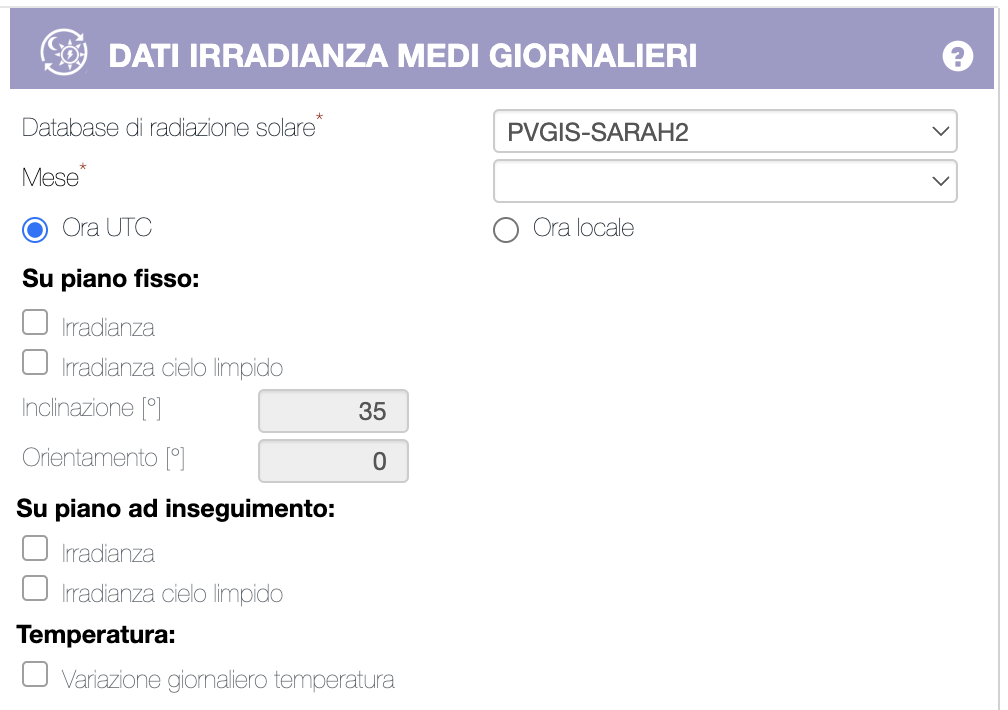
\includegraphics[height=0.5\textwidth]{res/cap 4/dati giornalieri}
    \caption{Scheda dati giornalieri}
\end{figure}\noindent
Tramite questa scheda una volta selezionato il mese che si intende valutare  ed il modello da utilizzare.
Questa scheda risulta molto comoda per confrontare soluzioni fisse con soluzioni ad inseguimento, per entrambe si possono ottenere dati sull'irradianza con cielo sia considerando che non la nuvolosità del cielo

\subsection{Export dati orario}
\label{subsec:export orario}
\begin{figure}[H]
    \centering
    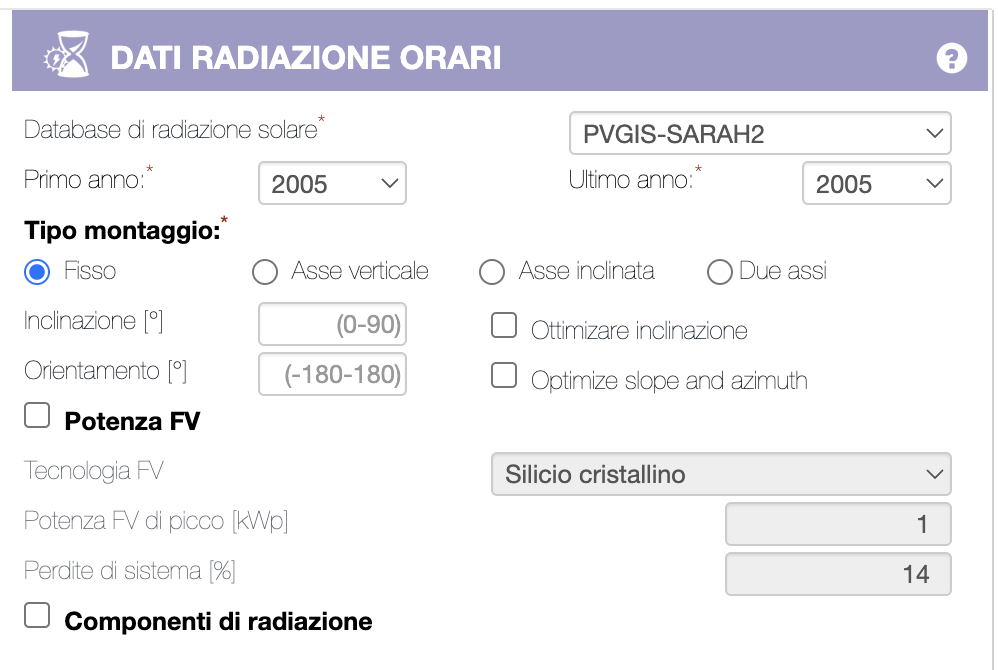
\includegraphics[height=0.5\textwidth]{res/cap 4/dati orari}
    \caption{Scheda dati orari}
\end{figure}\noindent
Tramite questa scheda una volta selezionato l'orizzonte temporaneo da prendere in analisi, il range disponibile dipende dal modello scelto, per quello presente in'immagine ad esempio sono presenti dati dal 2005 al 2020.
Prima di effettuare l'export bisogna selezionare il tipo di montaggio che si intende analizzare ed i parametri costruttivi.
Si ottiene in output un file contenente i vari timeframe, la potenza,l'irradianza nel piano scelto, l'altezza del sole,la temperatura dell'aria ed il vento a 10 metri dal suolo.
Spuntando anche l'output delle singole componenti si ottengono dati più dettagliati sulle componenti: diffusa, diretta e riflessa.

\subsection{Esempio di export di dati}
Sarà ora presentato un'esempio dei dati ottenibili per un'impianto fotovoltaico posizionato a terra in un terreno adiacente all'università.
Tutte le simulazione hanno in comune un grafico riportante l'orizzonte nelle diverse direzioni e l'angamento del sole, esso è molto utile per, ad esempio, poter effettuare una scelta più ponderata sull'orientazione dei moduli fotovoltaici.
\begin{figure}[H]
    \centering
    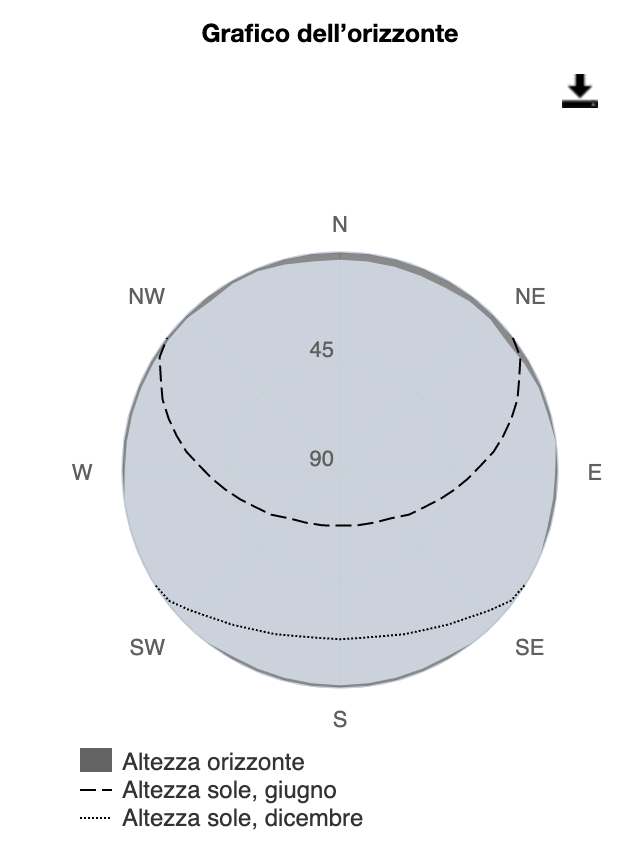
\includegraphics[height=0.5\textwidth]{res/cap 4/orizzonte}
    \caption{Diagramma contenente linea orizzonte ed altezza sole}
    \label{fig:orizzonte}
\end{figure}\noindent
Dal diagramma possiamo notare come la posizione scelta non subisca interferenza di ostruzioni naturali(montagne, colline), se si volesse tracciare anche l'interferenza di elementi più piccoli bisognerebbe inserire manualmente un profilo dell'orizzonte.
La simulazione sarà effettuata con per un'impianto tradizionale da 1Kwp inizialmente lasciando definire gli angoli di inclinazione e orientamento al software.
\begin{figure}[H]
    \centering
    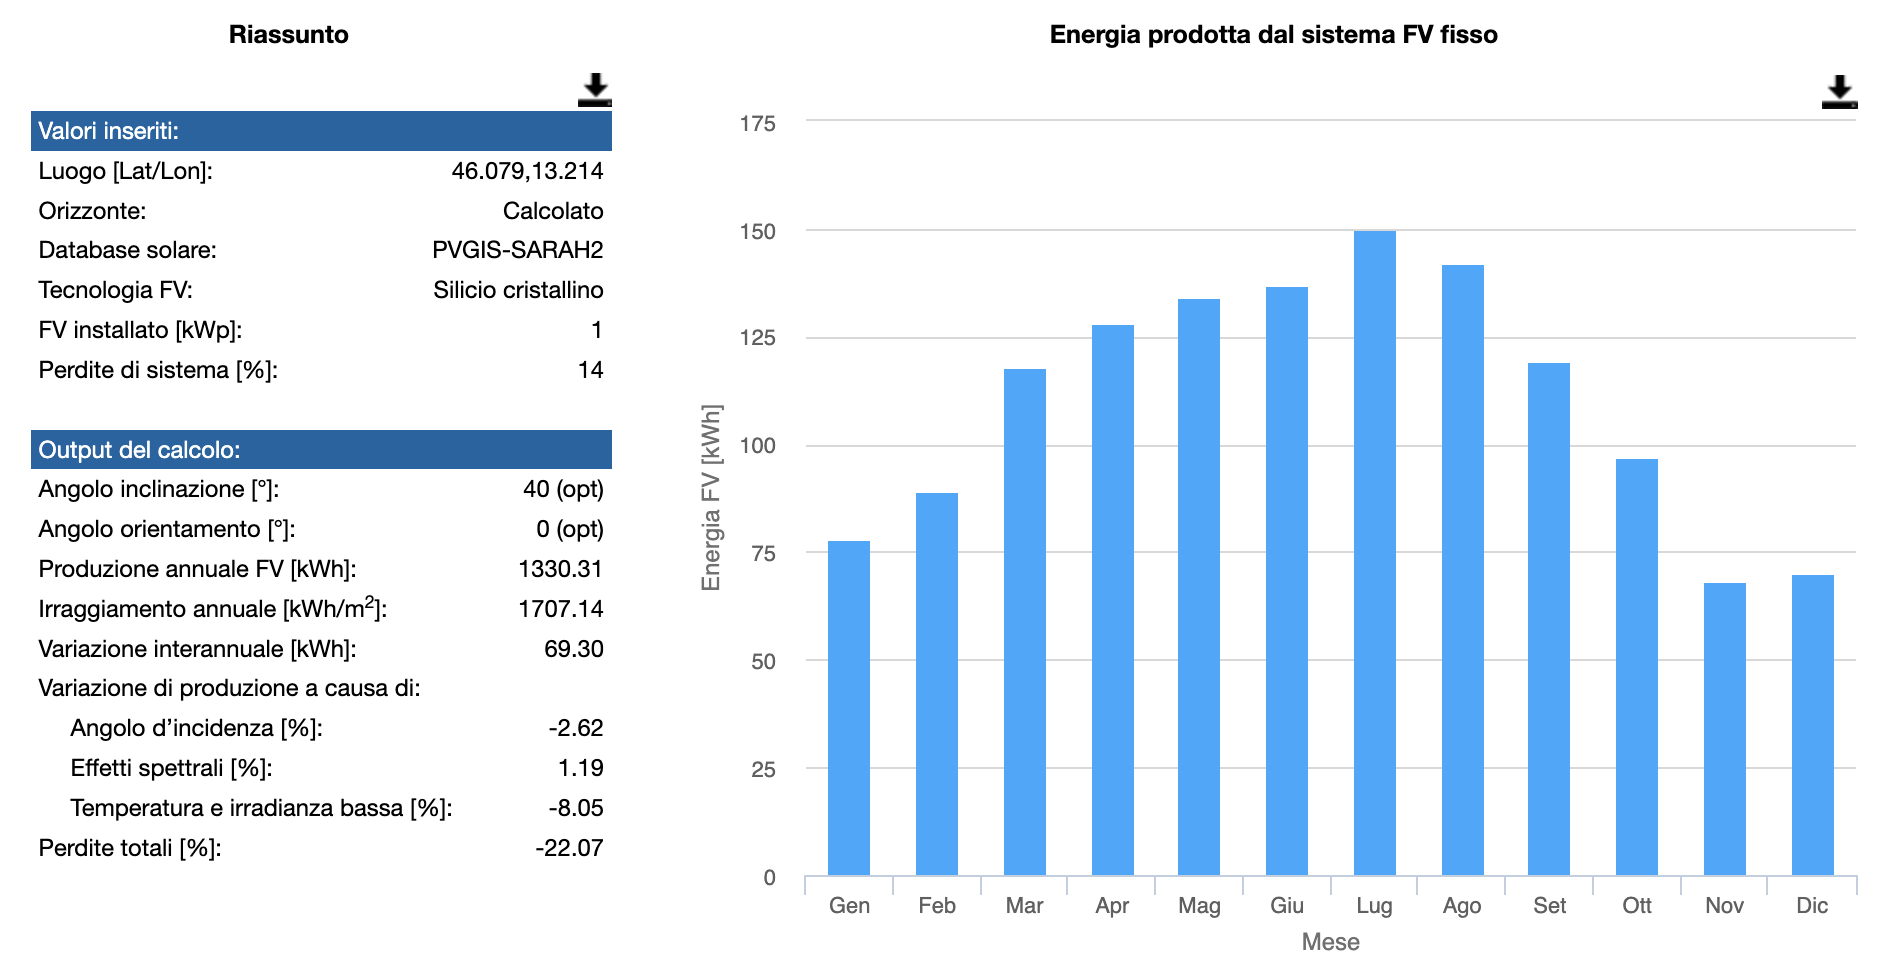
\includegraphics[height=0.5\textwidth]{res/cap 4/fissi uniud-auto}
    \caption{Export dati modulo fisso con orientazione automatica}
    \label{fig:export}
\end{figure}\noindent
Si può notare come il software abbia ovviamente orientato i moduli a sud, l'angolo è stato scelto per avere una resa media ottima in tutto l'anno.
Scegliere un'angolo minore incrementerebbe la produzione nei mesi estivi ma porterebbe un netto peggioramento in quelli invernali, un'inclinazione superiore ai 40 gradi invece gioverebbe nel periodo invernale ma sarebbe peggiorativa in quello estivo.
Procediamo ora con l'analisi di un'impianto ad inseguimento, lasciamo anche in questo caso al software la definizione degli angoli e in modo da poter confrontare nel caso ottimo le tre tipologie di impianti ad inseguimento.
\begin{figure}[H]
    \centering
    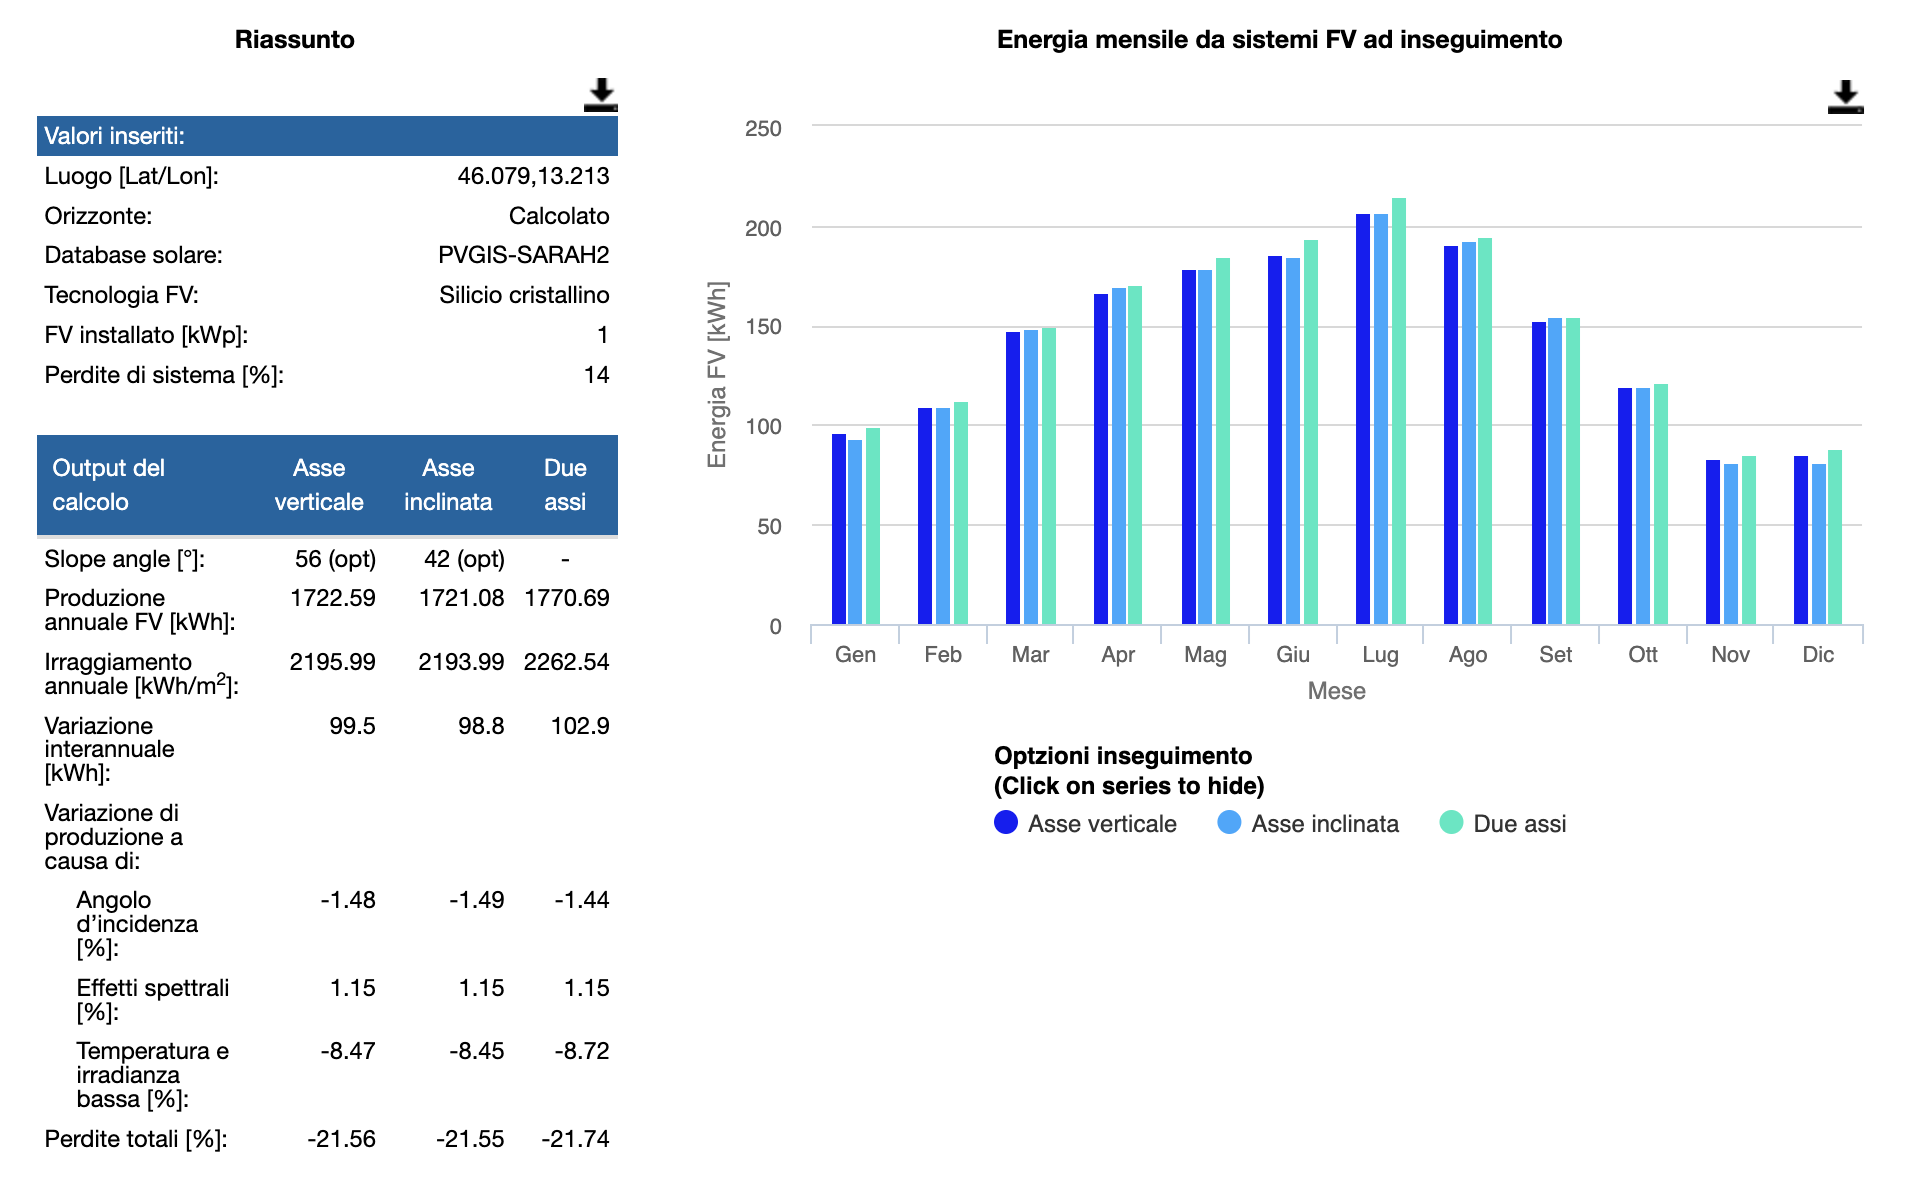
\includegraphics[height=0.6\textwidth]{res/cap 4/inseguimento uniud-auto}
    \caption{Export dati modulo fisso con orientazione automatica}
\end{figure}\noindent
Si nota come la produzione sia nettamente superiore al caso di moduli fissi e potendo orientare tutti gli assi ci sia un'ulteriore guadagno.
Il caso di impianto con accumulo non sarà trattato in quanto non di interesse per questa tesi.

    %!TEX root = ../main.tex

\chapter{Caso studio: comportamento campo fotovoltaico al variare della longitudine}
\label{chp:Caso studio: comportamento campo fotovoltaico al variare della longitudine}
Dopo un'attenta analisi dello strumento(PVGIS) l'obbiettivo di questo capitolo è stato quello di selezionare dieci luoghi a differenti latitudine tenendo fissata la longitudine del polo scientifico dell'università di udine.
\section{La selezione dei luoghi}
La selezione è avvenuta tenendo conto di diversi parametri oltre a quello sopraccitato, ogni regione è stata scelta cercando di attraversare ambienti diversi cercando di distribuire i punti in modo equo sul meridiano partendo da nord per arrivare fino all'equatore.
I parametri con i quali si è effettuata la scelta dei luoghi sono stati i seguenti:
\begin{itemize}
    \item rapporto tra radiazione diffusa e radiazione globale
    \item linea d'orizzonte libera sfruttando lo strumento in figura \ref{fig:orizzonte}
    \item analisi visiva del terreno per selezionare un luogo privo di impedimenti naturali od artificiali
    \item presenza di infrastrutture per il collegamento dell'ipotetico impianto
\end{itemize}
\noindent
Tutti questi parametri sono ovviamente stati calati alla singola regione in cui è stata effettuata l'analisi, in alcune regione desertiche ad esempio il rapporto tra radiazione diffusa e globale è particolarmente basso rispetto a quello che si può trovare ad esempio nelle regioni scandinave.
Per ogni luogo si è cercato di evitare di selezionare un ambiente con caratteristiche peculiari rispetto alla regione di appartenenza, andando ad eliminare luoghi che risulterebbero degli \enquote{outliers} andando a falsare i risultato dello studio.
\paragraph{I luoghi}\mbox{}\\
La scelta è ricaduta su 10 luoghi, ma maggior parte concentrati in Europa in quanto avente un clima vario anche a distanza di pochi chilometri:
\begin{table}[ht]
    \centering
    \begin{tabular}{|lll|}
    \hline
        \textbf{Location} & \textbf{Latitudine} & \textbf{Longitudine} \\ \hline
        Norvegia & 66.280 & 13.216 \\ \hline
        Svezia & 56.707 & 13.217 \\ \hline
        Germania & 52.211 & 13.215 \\ \hline
        Austria & 47.856 & 13.216 \\ \hline
        Friuli Venezia Giulia & 46.079 & 13.213 \\ \hline
        Lazio & 41.670 & 13.218 \\ \hline
        Sicilia & 37.527 & 13.210 \\ \hline
        Libia & 26.579 & 13.216 \\ \hline
        Nigeria & 12.470 & 13.214 \\ \hline
        Gabon & 0.739 & 13.211 \\ \hline
    \end{tabular}
    \label{tab:coordinate}
\end{table}
\begin{figure}[H]
    \centering
    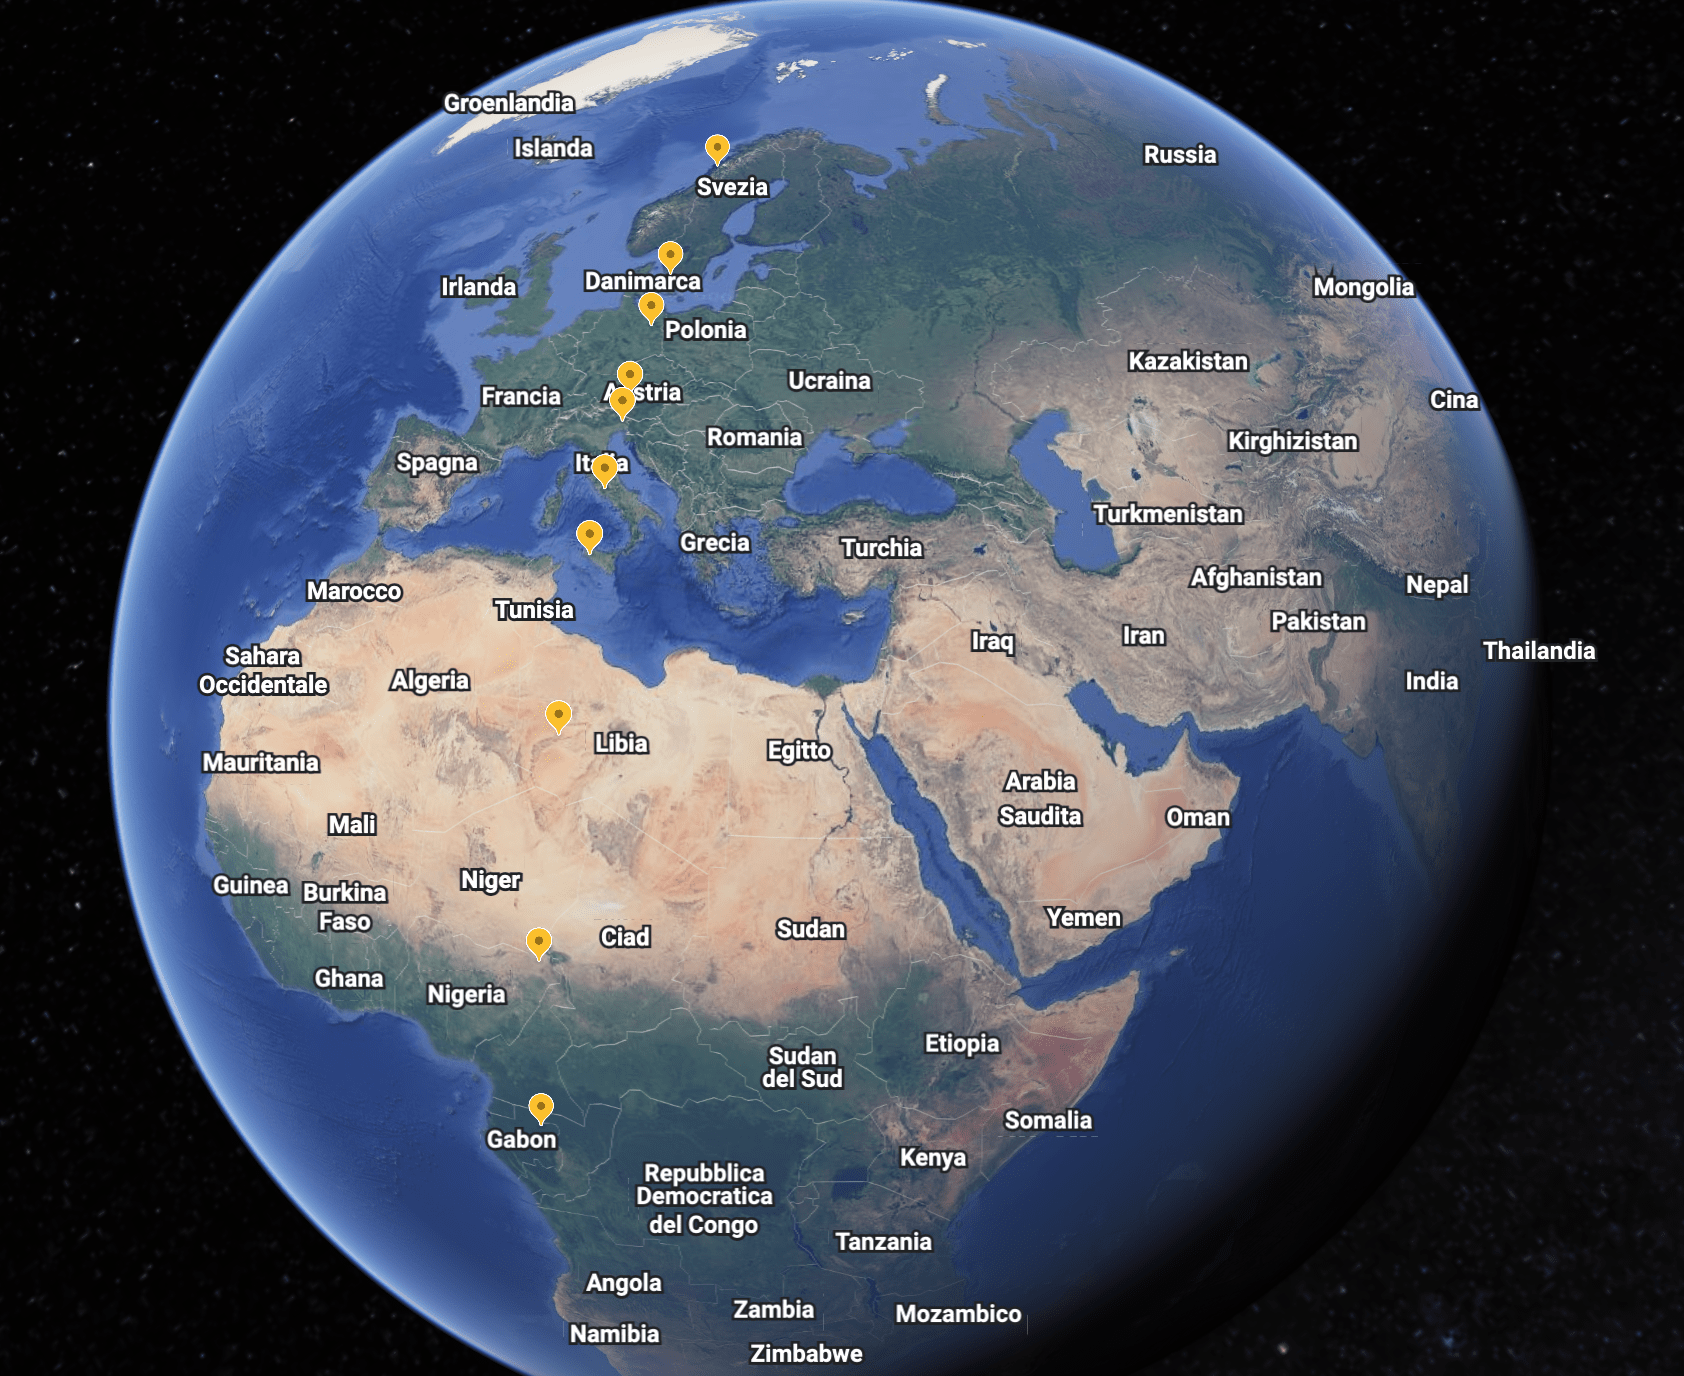
\includegraphics[width=0.9\textwidth]{res/cap 5/map.png}
    \caption{Mappa contenente luoghi scelti}
    \label{img:Mappa luoghi}
\end{figure}\noindent
Come visibile dalla mappa e dalla tabella soprastante i luoghi seguono quasi precisamente la stessa la longitudine e si collocano in 8 stati distinti.\\
Le maggiori difficoltà riscontate nella selezioni dei luoghi sono state sostanzialmente dovute ai seguenti motivi:
\begin{itemize}
    \item Nelle regioni nordiche il meteo varia molto velocemente quindi questo parametro purtroppo non è stato quasi considerato durante la selezione, la longitudine scelta attraversava a nord quasi solamente la zona dei fiordi portando quindi difficoltà nel trovare un'orizzonte libero
    \item Nella zona limitrofa all'arco alpino anche in questo caso la presenza di una catena montuosa ha generato zone di particolare nuvolosità ed anche in questo caso problemi dovuti alla ricerca di un'orizzonte libero
    \item Nella zona desertica invece i problemi sopraccitati non si sono ovviamente riscontrati dando invece origine ad un problema di trovare grossi agglomerati urbani o comunque zone popolate in cui collocare l'impianto
\end{itemize}
\noindent
\section{Simulazione}
In questa sezione tratterò l'analisi numerica dei singoli luoghi in modo da poter analizzare i dati raccolti nella successiva sezione.
La simulazione, come precedentemente anticipato, sarà effettuata su un impianto di \large{$1Kwp$} installato a terra e lasciando scegliere al software sia l'angolo di inclinazione che quello di orientamento, la perdita considerata sarà lasciata impostata al \large{$14\%$} in quanto ritenuto un valore medio di diferimento.\\
Per ogni location sarà quindi eseguita una simulazione simile a quella effettuata nel capitolo precedente in figura \ref{fig:export}.
Saranno inoltre inseriti dati statisti sul rapporto di diffusione(Kd) e sulla temperatura media,estratti dalla scheda in figura \ref{fig:export mensile}, considerando dati mensili tra il 2005 ed il 2020. I dati, come vedremo successivamente, saranno determinanti per valutare l'efficienza dell'installazione.\\
Successivamente saranno inseriti solo i luoghi che abbiano delle caratteristiche peculiari che può essere utile far notare.\\
\newpage
\subsection{Norvegia}
\begin{figure}[H]
    \centering
    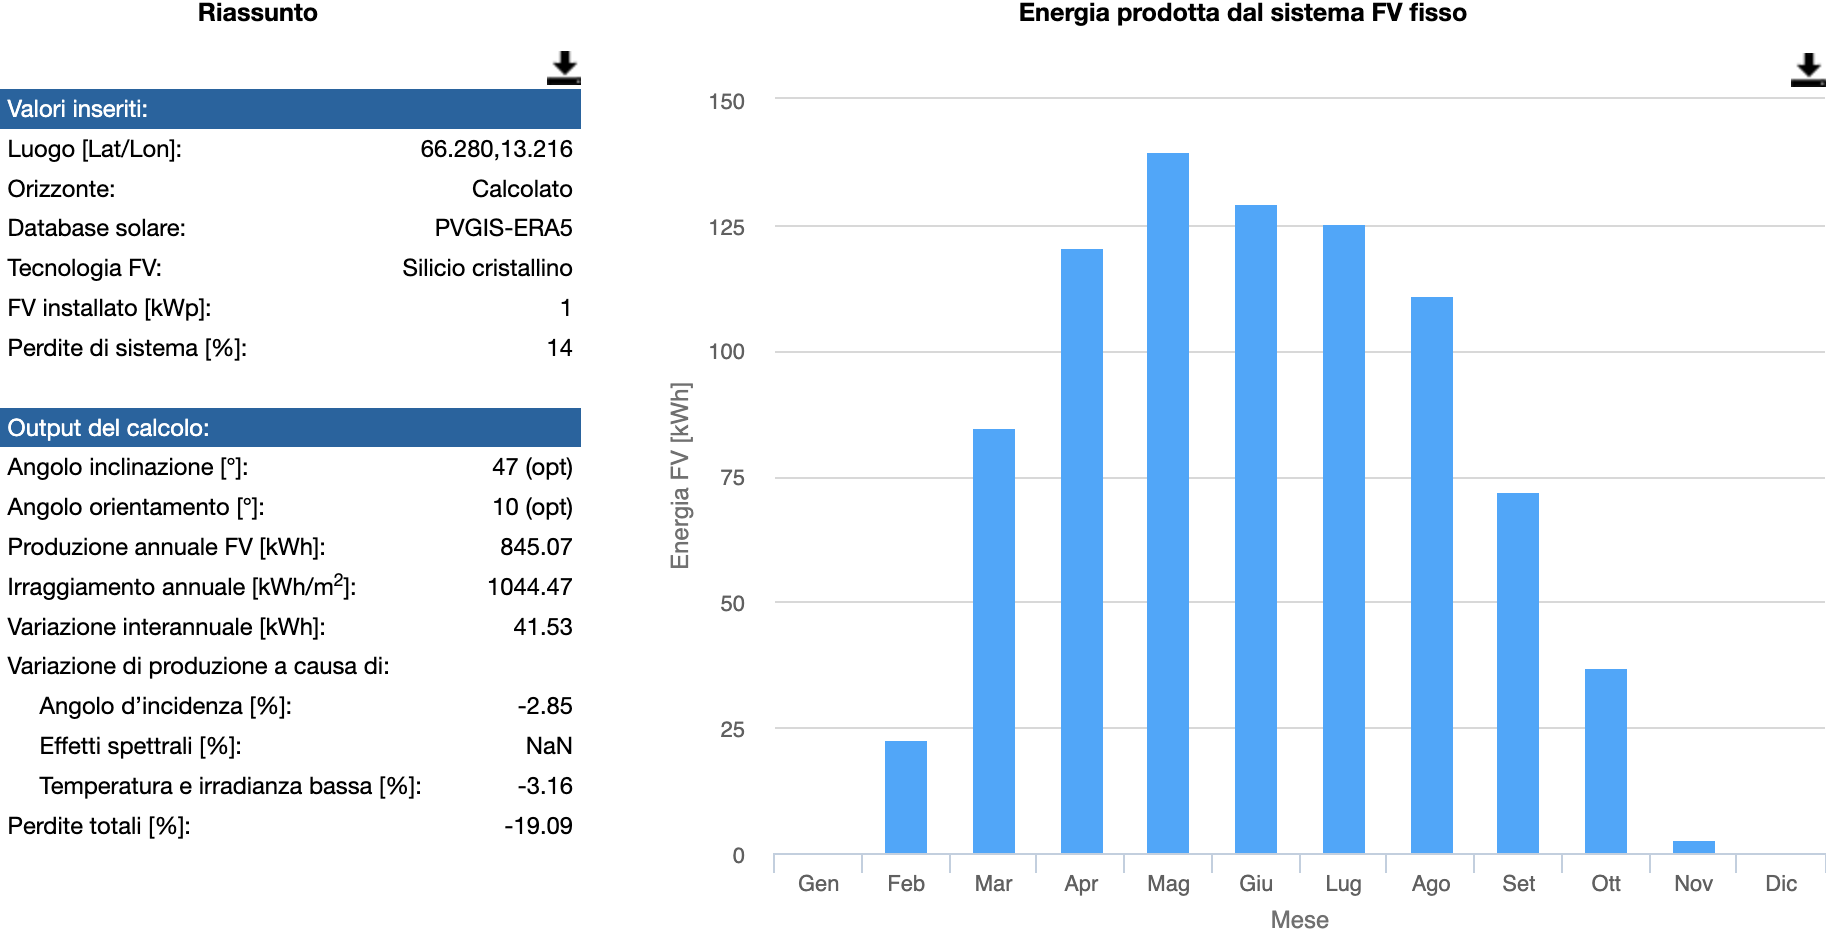
\includegraphics[width=0.7\textwidth]{res/cap 5/impianto norvegia}
\end{figure}\noindent
Come possiamo notare dai dai soprastanti in questo caso i moduli presentano un'angolo di inclinazione piuttosto elevato in quanto risulta l'unico modo per avere un buon rendimento ad latitudini elevate. Si nota come l'angolo di orientamento non sia esattamente zero, ciò è causato da un orizzonte a sud non perfettamente libero, risulta infatti trovato un'orizzonte più pulito a sud-ovest da qui i 10 gradi di orientamento.\\
A primo impatto si nota inoltre come la produzione nei mesi di novembre dicembre e gennaio sia pressocchè nulla, ciò è ovviamente dovuto alla notte polare, in quei mesi infatti il sole non sorgendo non permette ai moduli fotovoltaici di lavorare. Questo fenomeno man mano che ci si dirige verso sud viene sempre più attenuato.
Procediamo ora con un'analisi del Kd e della temperatura media:
\begin{table}[H]
    \centering
    \begin{tabular}{|l|l|l|}
    \hline
         & \textbf{Kd} & \textbf{Temp $[{}^\circ C]$} \\ \hline
        \textbf{Media} & 0,62 & 2,35 \\ \hline
        \textbf{Dev strd} & 0,23 & 7,33 \\ \hline
        \textbf{Mediana} & 0,54 & 1,50 \\ \hline
        \textbf{Massimo} & 1,00 & 18,60 \\ \hline
        \textbf{Minimo}  & 0,28 & -12,00 \\ \hline
    \end{tabular}
\end{table}\noindent
Dall'analisi numerica dei dati storici si nota come il Kd massimo trovato sia 1 ed è dovuto alla mancanza di radiazione diretta, la poca luce presente infatti è dovuta a sola componente diffusa.\\
La temperatura pur essendo il luogo scelto molto a nord risulta piuttosto e ciò può essere dato dalla vicinanza con un fiordo.
\vfill\newpage
\subsection{Friuli Venezia Giulia}
\begin{figure}[H]
    \centering
    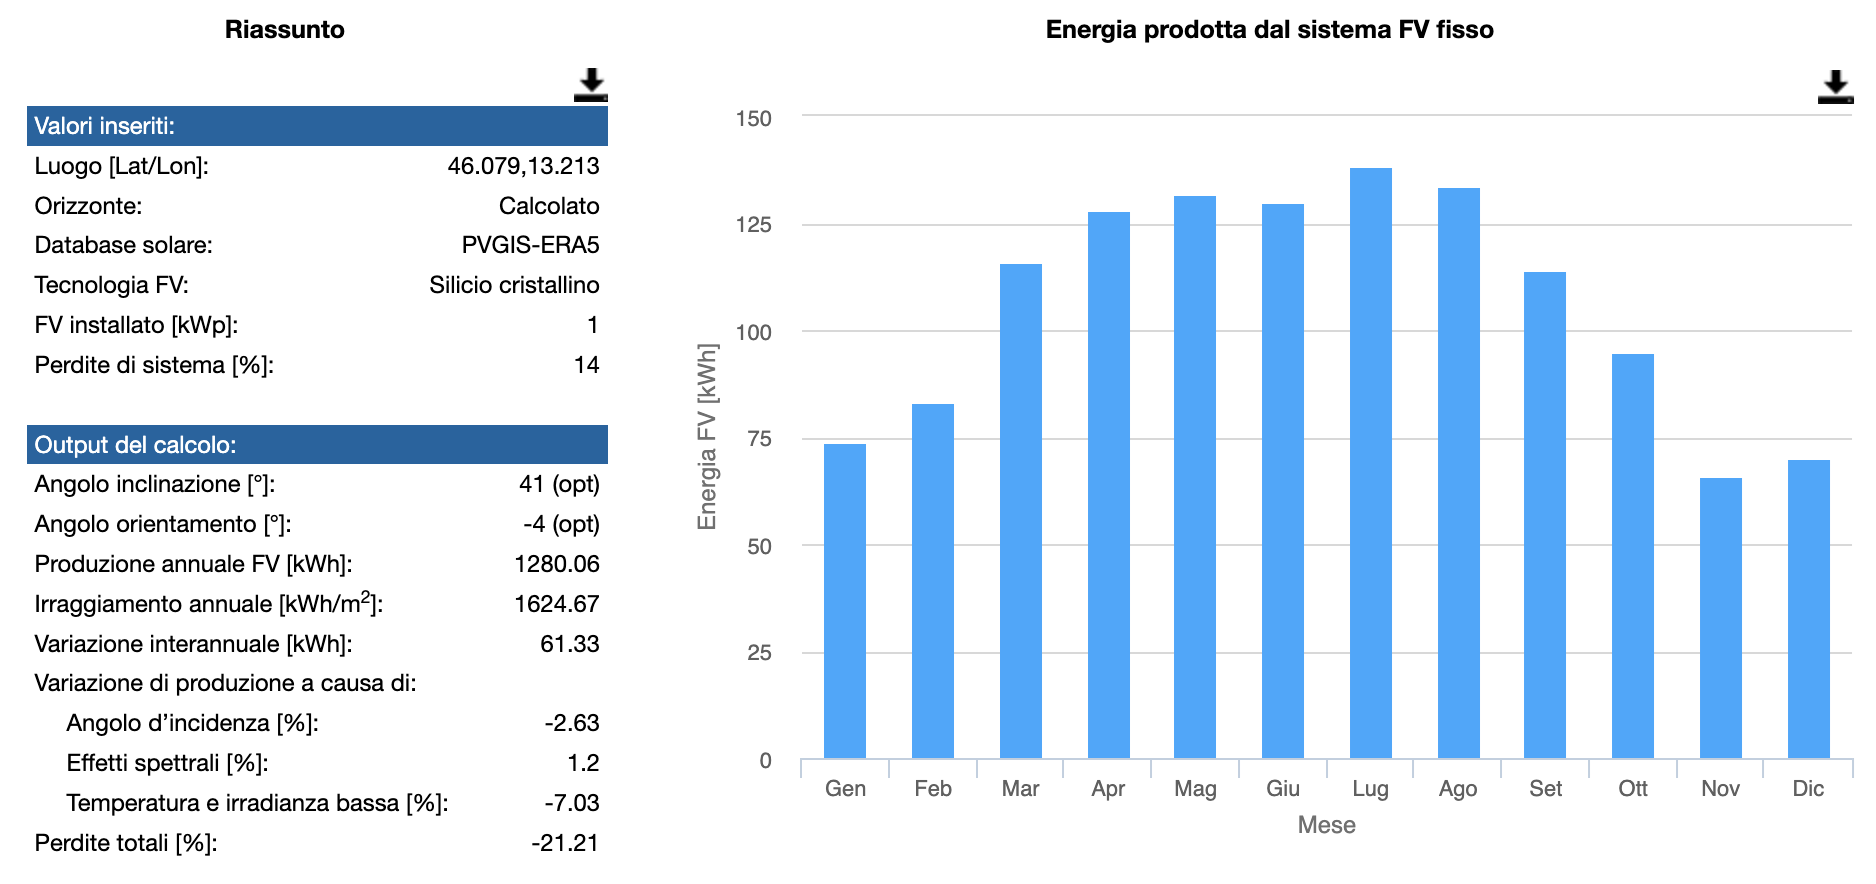
\includegraphics[width=0.7\textwidth]{res/cap 5/impianto udine}
\end{figure}\noindent
Come è possibile notare rispetto alla regione precedente l'angolo di inclinazione dei moduli è sceso con il diminuire della latitudine. La perdita relativa a temperatura e bassa irradianza risulta aumentata infatti come si può vedere dalla tabella sottostante la temperatura media è aumentata di ben 10 gradi rispetto all'estremo nord.\\
Il fenomeno che della notte polare è ovviamente del tutto sparito, ma permane una minor produttività dovuta sia al minor numero di ore di luce che all'arco che il sole compie all'orizzonte non garantendo un'angolo ottimale.\\
Aumentare l'angolo di inclinazione porterebbe infatti giovamento alle prestazioni nei mesi invernali peggiorando però la resa in quelli estivi, nel complesso la produzione annua sarebbe quindi minore.
\begin{table}[H]
    \centering
    \begin{tabular}{|l|l|l|}
    \hline	
          & \textbf{Kd} & \textbf{Temp $[{}^\circ C]$} \\ \hline
        \textbf{Media} & 0,38 & 12,66 \\ \hline
        \textbf{Dev strd} & 0,07 & 7,18 \\ \hline
        \textbf{Mediana} & 0,38 & 12,50 \\ \hline
        \textbf{Massimo} & 0,60 & 25,90 \\ \hline
        \textbf{Minimo} & 0,25 & 0,20 \\ \hline
    \end{tabular}
\end{table}
Il coefficiente diffusione è calato a causa della presenza di un clima più mite ed una minor nuvolosità, i fenomeni che nel nord Italia portano questo parametro a non essere comunque ottimale sono l'elevata presenza di particelle in sospensione nell'ora che portano a fenomeni di diffusione.
\vfill
\newpage
\subsection{Libia}
\begin{figure}[H]
    \centering
    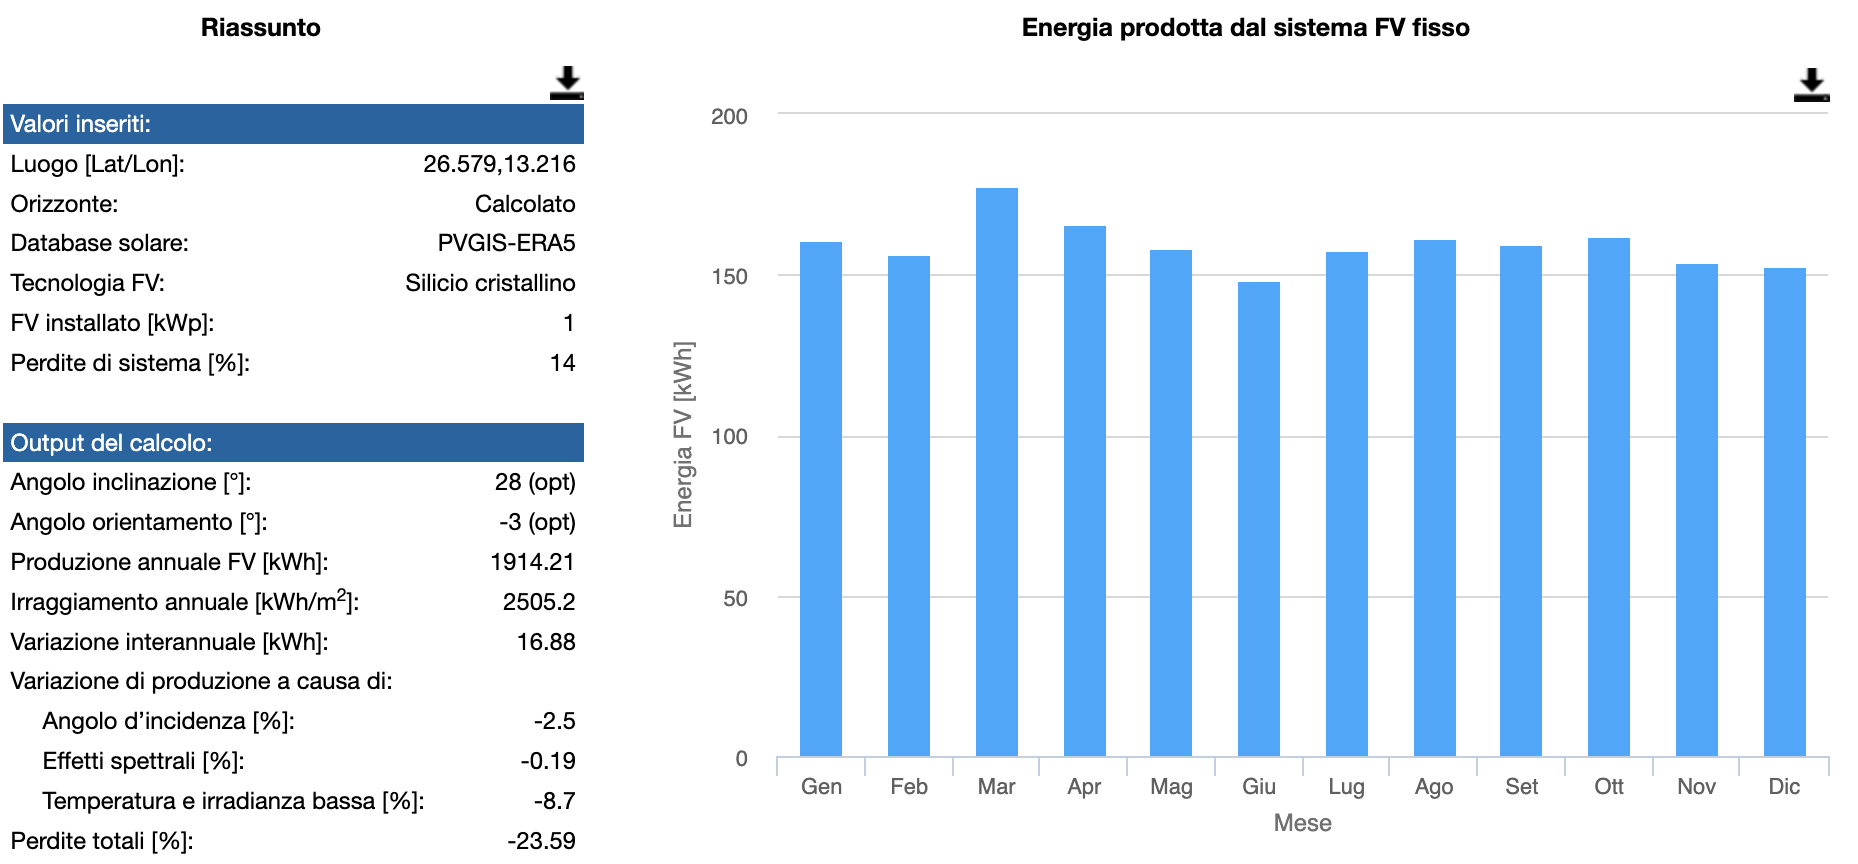
\includegraphics[width=0.7\textwidth]{res/cap 5/impianto libia}
\end{figure}\noindent
L'avvicinamento all'equatore è subito visibili dalla netta diminuzione dell'angolo di inclinazione, non vi è praticamente più una differenza sostanziale tra i vari periodi dell'anno e ciò è ovviamente dovuto ad una minor differenziazione delle stagioni.\\
La produzione risulta ridotta a causa della temperatura che è ovviamente maggiore rispetto alle regioni viste in precedenza e ciò è dovuto alla presenza di un clima sostanzialmente desertico.
\begin{table}[H]
    \centering
    \begin{tabular}{|l|l|l|}
    \hline
          & \textbf{Kd} & \textbf{Temp $[{}^\circ C]$} \\ \hline
        \textbf{Media} & 0,24 & 22,99 \\ \hline
        \textbf{Dev strd} & 0,03 & 7,78 \\ \hline
        \textbf{Mediana} & 0,24 & 22,99 \\ \hline
        \textbf{Massimo} & 0,34 & 33,40 \\ \hline
        \textbf{Minimo} & 0,20 & 8,90 \\ \hline
    \end{tabular}
\end{table}
Il coefficiente di diffusione in questo caso è particolarmente basso e costante, anche qui grazie alla presenza di un clima desertico, la temperatura media e massima per lo stesso motivo si alza notevolmente.
\vfill\newpage
\subsection{Gabon}
\begin{figure}[H]
    \centering
    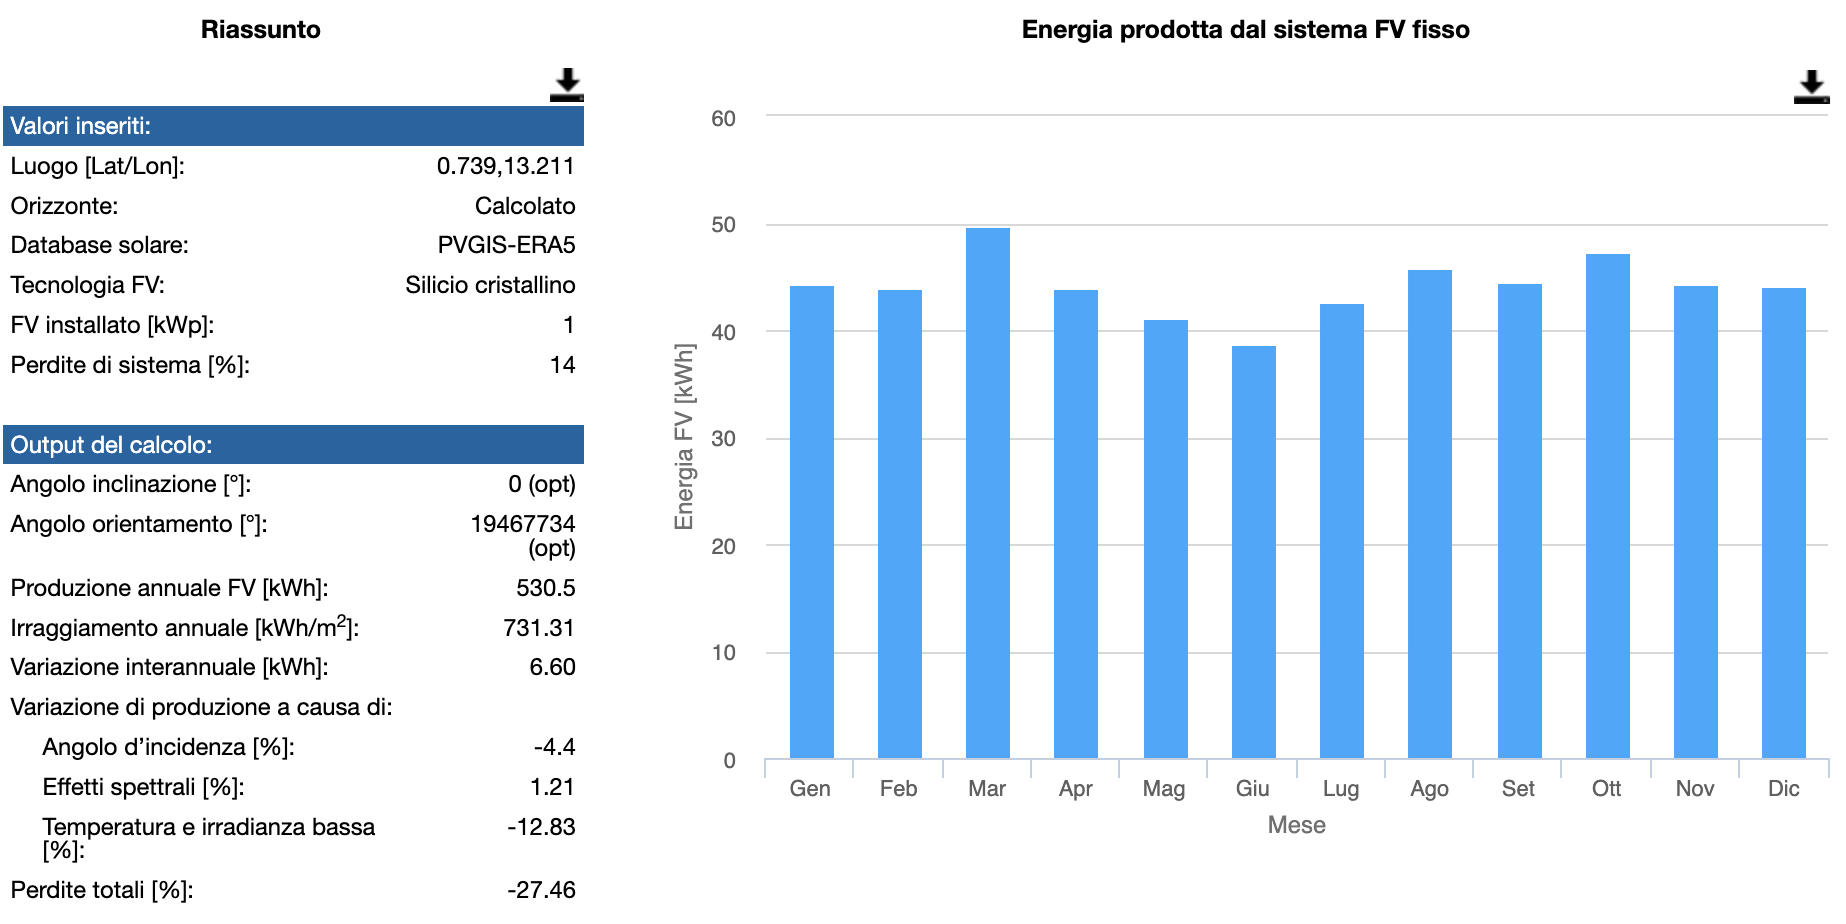
\includegraphics[width=0.7\textwidth]{res/cap 5/impianto gabon}
\end{figure}\noindent
Osservano i dati riguardanti il posizionamento si osserva che l'inclinazione in questo caso è di 0 gradi essendo la componente diretta proveniente già da una direzione perpendicolare. Per quanto riguarda l'orientazione viene erroneamente calcolata in quando per un pannello disposto con un angolo di 0 gradi sul terreno non può essere espresso .\\
In questa regione si nota un fenomeno particolare, ci si aspetterebbe infatti che la zona equatoriale sia quella che riceve una radiazione solare più intensa tuttavia a causa di una non uniforme della radiazione ciò non è del tutto vero.\\
Un altro fenomeno che fa si che l'anello equatoriale scarsamente irradiata è la presenza quasi costante di nuvole e quindi una scarsa componente diretta a favore di una componente diffusa e quindi meno efficace.\\
In un ambiente con le caratteristiche appena viste potrebbe essere interessante utilizzare dei moduli fotovoltaici che presentino una struttura cristallina non orientata la quale garantirebbe una maggior efficienza in caso di componente diffusa altamente presente.
\begin{table}[H]
    \centering
    \begin{tabular}{|l|l|l|}
    \hline	
          & \textbf{Kd} & \textbf{Temp $[{}^\circ C]$} \\ \hline
        \textbf{Media} & 0,45 & 24,44 \\ \hline
        \textbf{Dev strd} & 0,04 & 0,56 \\ \hline
        \textbf{Mediana} & 0,45 & 24,44 \\ \hline
        \textbf{Massimo} & 0,55 & 26,40 \\ \hline
        \textbf{Minimo} & 0,34 & 23,30 \\ \hline
    \end{tabular}
\end{table}
La presenta di un clima particolare è chiaramente evidente osservano i valori statistici ottenuti. Il valore minimo di Kd infatti risulta il maggiore trovato in tutte le regioni precedenti e questo è indice di un clima non ottimale, si riscontra in oltre una media elevata ed una bassa variabilità il che è indice di alta diffusione che permane nel tempo.\\
La temperatura,anche a causa della nuvolosità, risulta più alta ma con massimi più bassi ed una deviazione standard molto più bassa di tutte le regioni desertiche viste in precedenza.Queste caratteristiche sono molto indicative della situazione climatica della regione\\
\section{Analisi e conclusione}
Terminata la descrizione delle singole location è possibile confermare le aspettative iniziali:
\begin{itemize}
    \item Andando verso la zona equatoriale i moduli fotovoltaici avrebbero mantenuto l'orientamento il più possibile a sud e l'inclinazione sarebbe diminuita progressivamente
    \item La presenza di climi caldi ha favorito la riduzione del Kd garantendo quindi un maggior presenza di componente diretta rispetto a quella diffusa
    \item L'aumento della temperatura ha peggiorato tendenzialmente la resa del moduli fotovoltaici ma tale peggioramento è stato irrilevante in quanto l'aumento delle ore di sole ha mitigato notevolmente il problema
\end{itemize}
A differenza delle aspettative iniziali la zona equatoriale non si è rivelata la migliore in cui installare un campo fotovoltaico a causa del fenomeni citati in precedenza.
Compresa l'importanza fondamentale di avere un modulo correttamente orientato ho provveduto a studiare l'angolo ottimale cercando una correlazione con la latitudine e come mi aspettavo ho ottenuto il seguente risultato:
\begin{figure}[H]
    \centering
    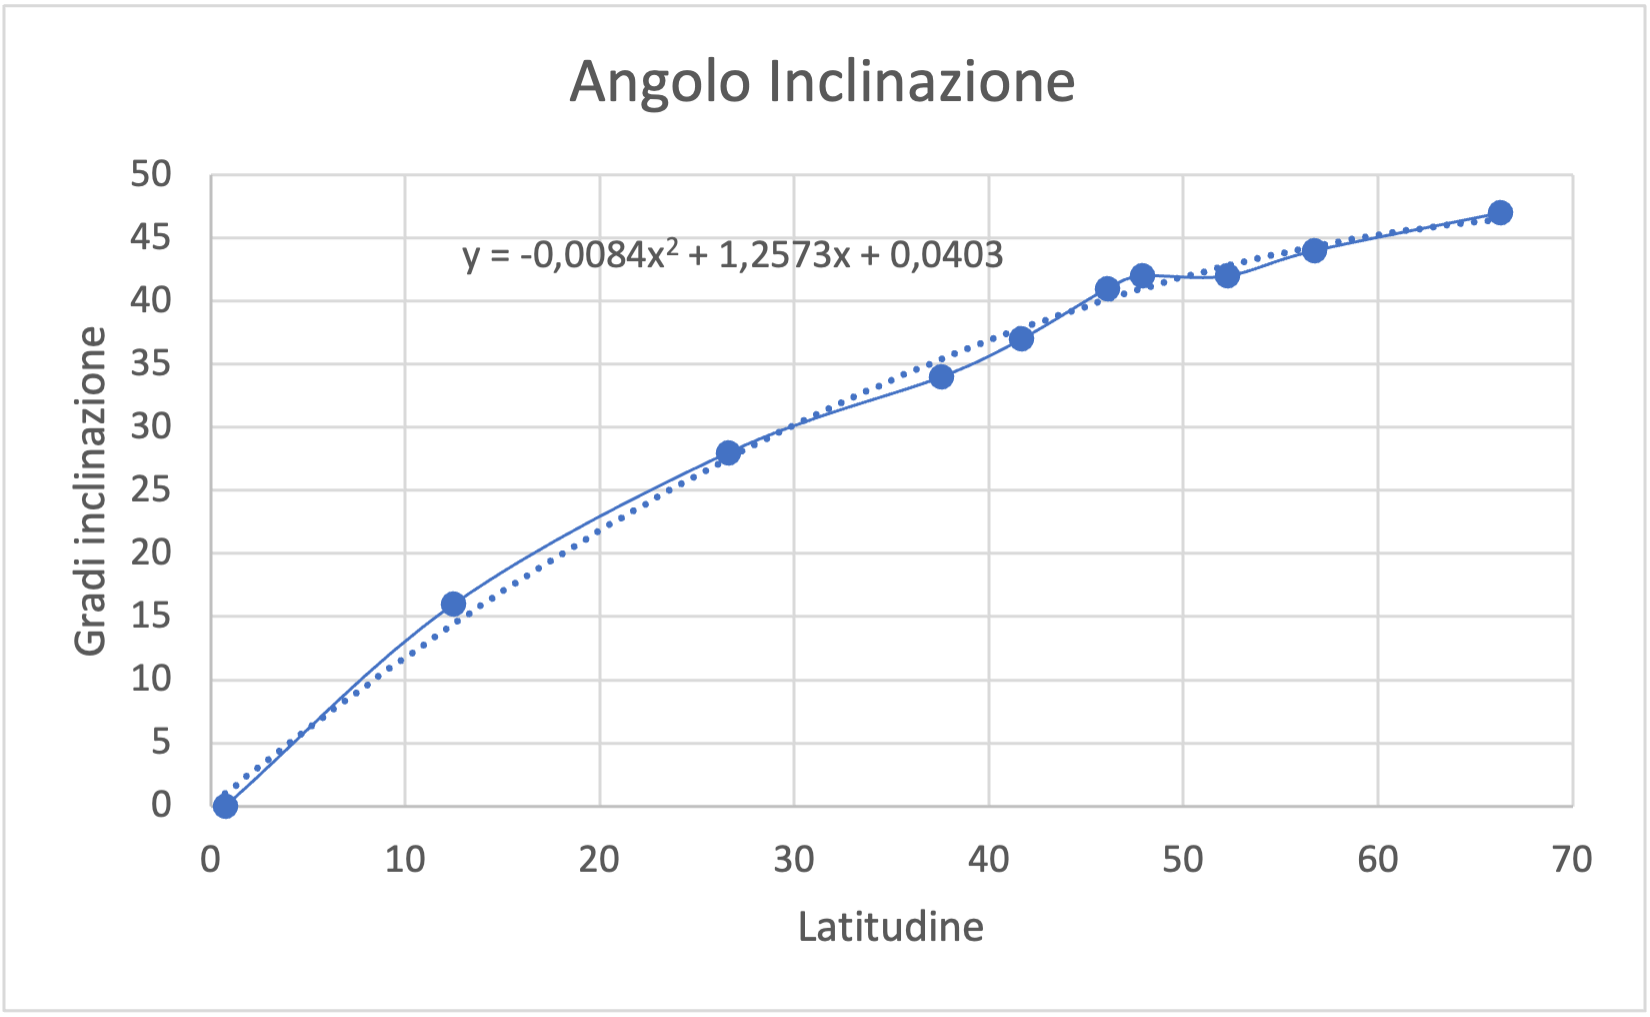
\includegraphics[width=0.8\textwidth]{res/cap 5/regressione lineare}
    \caption{Regressione lineare utilizzando i dati dei luoghi campione}
\end{figure}\noindent
A primo impatto era subito chiaro che vi fosse una funziona di secondo grado che potesse, a partire dalla latitudine, generare l'angolo di inclinazione ottimale. Ho provveduto quindi ad inserire la funzione di regressione lineare ed a graficarla ottenendo la seguente formula:
\begin{center}
    \large{$Angolo\space di\space inclinazione = -0,0084 \cdot (lat)^2 + 1,2573\cdot lat + 0,0403$}
\end{center}
\noindent
Ho provveduto quindi a testare sempre attraverso il tool PVGIS la formula sopra indicato ottenendo un quasi ottimale funzionamento in tutto l'emisfero boreale ad esclusione dei punti più limitrofi al polo nord ma di scarso interesse applicativo in quanto scarsamente popolati e, come visto nel capitolo, non idonei ad ospitare campi fotovoltaici.\\
Per ottenere allo stesso modo un modello capace di restituire l'inclinazione ideale per l'emisfero australe sarebbe sufficiente raccogliere una serie di dati e ripetere la regressione lineare con il nuovo dataset scelto.
    \chapter{Conclusioni}
\label{chp:Conclusioni}
Data la necessita sempre più impellente di virare la produzione energetica verso tecnologie più sostenibili per l'ambiente, sono stati presi in analisi nello specifico gli impianti rinnovabili. Da questa ho potuto osservare come spesso si faccia riferimento solo all'inquinamento diretto prodotto da un impianto senza però considerare tutti i fattori di inquinamento indiretti.
Ci troviamo spesso davanti ad impianti che hanno un alto impatto paesaggistico e per la fauna generando impedimenti architettonici o variazioni dell'ambiente naturale tali da alterarne le proprietà.\\
Un ulteriore fattore che rende molto difficile questa transizione ecologica è l'impossibilità di prevedere e controllare la produzioni delle centrali a causa dell'irregolarità dei fenomeni meteorologici. Fenomeni che non essendo costanti e distribuiti in modo uniforme sulla terra rendono solo un numero ridotto di luoghi adatti ad ospitare uno specifico impianto.\\
Stiamo vivendo un momento storico nel quale il meteo è sempre più irregolare con, ad esempio, forti fenomeni piovosi e lunghi periodi di siccità. Caratteristiche che sono totalmente inadeguate in un mondo in cui la richiesta energetica è costante ed in crescita.\\
Nel capitolo finale sono state prese in analisi le caratteristiche di un impianto fotovoltaico ponendolo sempre nelle condizioni di lavoro ottimali rispetto al suo posizionamento geografico. Spesso ci si trova, per ridurre fenomeni di larga occupazione del suolo, ad installare il fotovoltaico su superfici non ideali quali ad esempio tetti di edifici dell'agglomerato urbano.
Lo scopo di queste installazioni è quello di cercare di far avvicinare la domanda di energia con la produzione andando a sfruttare spazi che in caso contrario sarebbero stati inutilizzati. Risulta facilmente intuibile come l'installazione superfici esistenti risulti difficoltosa od a volte addirittura poco conveniente data la scarsa resa di piani non correttamente inclinati ed orientati.\\
Ci troviamo di fronte ad una situazione quindi molto difficile in quanto è assolutamente necessario procedere con una veloce decarbonizzazione per ridurre il costante incremento della temperatura globale e mitigare i cambiamenti climatici. Per perseguire questa strada però difficilmente sarà possibile utilizzare solo fonti rinnovabili per come sono tecnologicamente concepite nel periodo odierno.
    
    % Bibliography, appendix, acknowledges, etc...
    \backmatter
\end{document}